\documentclass[]{article}
\usepackage{amsmath}
\usepackage{amsfonts}
\usepackage{amssymb}
\usepackage{hyperref}
\usepackage{gensymb}
\usepackage{graphicx}
\usepackage{svg}
\usepackage{bbding}
\usepackage{mathtools}
\usepackage{centernot} % not parallel, etc.
\usepackage{lmodern}
\usepackage{morewrites}
\usepackage{xcolor,sectsty} % colorful sections
\usepackage[left=10mm, top=10mm, right=10mm, bottom=20mm, nohead]{geometry}
%\usepackage{bigints}
\usepackage{dsfont} %mathbb 1
\usepackage{esint} % beatiful integrals
\usepackage{physics}


\DeclareFontFamily{OMX}{lmex}{}
\DeclareFontShape{OMX}{lmex}{m}{n}{<-> lmex10}{}


%colors of sections
\definecolor{secfont}{RGB}{46,116,181}
\definecolor{subfont}{RGB}{146,23,57}
\definecolor{parfont}{RGB}{19,127,43}
\definecolor{subparfont}{RGB}{7,11,100}

\subsectionfont{\color{subfont}}
\sectionfont{\color{secfont}}
\paragraphfont{\color{parfont}}
\subparagraphfont{\color{subparfont}}

%\usepackage{babel}[english]
%opening
\title{104030 - Introduction to Partial Differential Equations}
\author{Gershon Velinski}

\parindent=0em
\begin{document}


\maketitle

\begin{abstract}

\end{abstract}

%\tableofcontents
\section{Introduction}
\paragraph{PDE}
In PDE, the solution is a function of a couple of variables $u(x_1, x_2, \dots x_m)$ such that:
$$F(x_1, x_2, \dots x_m, u_{x_1}, u_{x_2}, \dots, , u_{x_m}, u_{x_1x_1}, \dots) = 0$$
Notation is 
$$u_{x_i} = \frac{\partial u}{\partial x_i}$$
Usually $m=2$. For example
$$F(x_1,x_2, u, u_{x_1}, u_{x_2}, u_{x_1x_1}, u_{x_2x_2}, u_{x_1x_0}) = 0$$
Is PDE of two variables of order 2.
\paragraph{Linear PDE}
PDE is linear if $F$ is linear in $u$ and its derivatives. First order linear PDE is
$$F(x_1,x_2, u, u_{x_1}, u_{x_2}) = a(x_1,x_2)u_{x_1} + b(x_1,x_2)u_{x_2} + c(x_1,x_2)u + d(x_1,x_2) = 0$$
Second order linear PDE is
\begin{align*}
F(x_1,x_2, u, u_{x_1}, u_{x_2}, u_{x_1x_1}, u_{x_1x_2}, u_{x_2x_2}) =\\= A(x_1,x_2) u_{x_1x_1} + B(x_1,x_2) u_{x_1x_2} + C(x_1,x_2) u_{x_2x_2} + a(x_1,x_2)u_{x_1} + b(x_1,x_2)u_{x_2} + c(x_1,x_2)u + d(x_1,x_2) = 0
\end{align*}
\paragraph{Quasilinear PDE}
Quasilinear PDE is linear only in highest order derivative. First order quasilinear PDE:
$$F(x_1,x_2, u, u_{x_1}, u_{x_2}) = a(x_1,x_2, u)u_{x_1} + b(x_1,x_2, u)u_{x_2} + c(x_1,x_2, u) = 0$$
And second order one:
\begin{align*}
F(x_1,x_2, u, u_{x_1}, u_{x_2}, u_{x_1x_1}, u_{x_1x_2}, u_{x_2x_2}) =\\= A(x_1,x_2, u, u_{x_1}, u_{x_2}) u_{x_1x_1} + B(x_1,x_2, u, u_{x_1}, u_{x_2}) u_{x_1x_2} + C(x_1,x_2, u, u_{x_1}, u_{x_2}) u_{x_2x_2} + g(x_1,x_2, u, u_{x_1}, u_{x_2}) = 0
\end{align*}

For homogeneous linear PDE solution always exist. In addition, if $u_1$, $u_2$, then any linear combination of those $\lambda_1 u_1 + \lambda_2 u_2$ will also be a solution. Thus set of solutions of linear homogeneous PDE is vector space.

\paragraph{Autonomous PDE } If $F$ is independent on $x_i$, then if $u(x_1, \dots, x_i, \dots, x_m)$ is solution then $u(x_1, \dots, x_i+\lambda, \dots x_m)$ is solution too. 

In particular if $u$ is independent on all $x_i$, then $u(x_1+\lambda_1, \dots, x_i+\lambda_i, \dots, x_m+\lambda_m)$.

\subsection{Wave equation}
$$u_{tt} - c^2 u_{xx} = 0$$
Solution describes movement of wave.

Lets start ODE describing harmonic oscillator, would be
$$m \frac{d^2x}{dt^2} = k(x - x_0)$$

Now suppose that we have $N$ such masses and positionn of mass is $\bar{x}_i = x_i+u(x_i, t)$, where $u$ is displacement of mass and $x_i - x_{i-1} = \Delta$. Then the position of mass is described as
$$\frac{\partial \bar{x}_i}{\partial t^2} = m\frac{\partial^2 }{\partial t^2}u(x_i,t) = k(\bar{x}_{i+1}-\bar{x}_i)+k(\bar{x}_{i}-\bar{x}_{i-1})$$
Thus
$$m\frac{d}{dt^2}u(x,t) = k \left[ u(x_{i+1},t) - 2u(x_i,t) + u(x_{i-1},t) \right]$$
In limit $\Delta \to 0$:
$$\frac{d}{dt^2}u(x,t) = c^2\frac{d}{dx^2}u(x,t)$$
Where
$$c^2 = \lim_{\Delta \to 0} \frac{\Delta^2 k_\Delta}{m_\Delta} $$
\paragraph{Possible solutions}
For each function $f$ in $\mathcal{C}^2$, $u=f(x-ct)$ is a solution of wave equation:
$$\begin{cases}
u_{xx} = f''(x-ct)\\
u_{tt} = c^2 f''(x-ct)
\end{cases}$$

This solution is moving wave, because it moves along $x$ axis with constant velocity $c$. Since $c$ can be negative too, we have solution
$$u(x,t) = f(x+ct) + g(x-ct)$$
\subsection{Heat equation}
$$\frac{\partial u}{\partial t} = k \frac{\partial^2 u}{\partial x^2} $$
Here, $u$ means amount of heat in point $x$ at time $t$.

Amount of heat in interval $[a,b]$ is
$$Q(t) = \int_a^b u(x,t) dx$$
And heat flux in point $x$ at time $t$ is $k\frac{\partial u}{\partial x}$

Then flux out of interval is
$$\frac{dQ}{dt} = k\frac{\partial u}{\partial x}(b,t) - k\frac{\partial u}{\partial x}(a,t)$$
Thus
$$\int_a^b \frac{\partial }{\partial t}u(x,t) dx  = k\frac{\partial u}{\partial x}(b,t) - k\frac{\partial u}{\partial x}(a,t)$$
In limit $b\to a$ we get
$$\frac{\partial u}{\partial t} = k \frac{\partial^2 u}{\partial x^2} $$

\paragraph{Example solution}
$$u(x,t) = e^{-kst} \sin (\sqrt{s} x)$$
for some parameter $s$. Here we also can add some constant to $x$ and acquire additional solution:
$$U(x,t) = e^{-kst} \sin (\sqrt{s} (x+\lambda)) = \cos (\sqrt{s} \lambda ) e^{-kst} \sin (\sqrt{s} x) +  \sin (\sqrt{s} \lambda ) e^{-kst} \cos (\sqrt{s} x)$$
Thus
$$w(x,t) =  e^{-kst} \cos (\sqrt{s} x)$$
is solution too.
\subsection{Diffusion equation}
Suppose
$u(x_1,x_2,x_3,t)$ describes concentration of material in space. From continuity:
$$\frac{\partial u}{\partial t} + \vec{\nabla} \cdot (\vec{v} u) = 0$$
$$\frac{\partial u}{\partial t} +\frac{\partial }{\partial x_1} (\vec{v} u) +\frac{\partial }{\partial x_2} (\vec{v} u) +\frac{\partial }{\partial x_3} (\vec{v} u) = 0$$
for some vector field $v$ independent on $u$.
\subsection{Elliptic PDEs}
\paragraph{Laplace equation}
$$\Delta u = \frac{\partial^2 u}{\partial x_1^2} + \frac{\partial^2 u}{\partial x_2^2} = 0$$
\paragraph{Poisson equation}
$$\Delta u = f(x_1,x_2)$$
\section{First-order PDE}
$$\frac{\partial u}{\partial t} + c\frac{\partial u}{\partial x} = 0$$
We can easily guess solution similarly to wave equation: $u(x,t) = f(x-ct)$ for some differentiable $f$. 

Suppose we have initial conditions $u(x,0)= u_0(x)$. Is it determines uniquely a solution of equation? Obviously, $u(x,t) = u_0(x-ct)$ is a solution.

Lets show it's unique. Take a look at parametrization $x(t) = s_1 + ct$.
$$\frac{d}{dt} u(x(t),t) = c\frac{\partial u}{\partial x}(x(t),t) + \frac{\partial u}{\partial t}(x(t),t) = 0$$ 
Thus $u$ is constant on every line of form $x(t)=s+ct$. Such lines are called characteristic curves or just characteristics. Thus if we know a value of $u$ in some point on a line, we know it on the whole line.

\paragraph{} Is it possible to find a solution if we are given initial conditions for some curve $x(t)$ for $t \in [a,b]$. So we want to find a solution such that the surface of solution comprises a given curve in 3D.

The solution exists if the curve of initial conditions doesn't merges with characteristic line, we have a unique solution. If it does, either there is no solution, or there are infinite number of solution.

\subsection{Quasilinear first-order equations}
$$a(x,y,u)u_x + b(x,y,u)u_y = c(x,y,u)$$
where $a,b,c$ are continuously differentiable in some neighborhood of point $(x_0,y_0,z_0)$.

Take a look at
$$f(x,y,z) = z - u(x,y)$$
$$\nabla f = \left(-\frac{\partial u}{\partial x},-\frac{\partial u}{\partial y},1\right)$$
and
$$\nabla f \cdot (a,b,c) = -a\frac{\partial u}{\partial x} -b\frac{\partial u}{\partial y}+c  = 0$$
Thus vector $(a,b,c) $ is tangent to solution surface.

Now define curve such that
$$\begin{cases}
\frac{dx}{dt} = a(x(t), y(t), z(t))\\
\frac{dy}{dt} = b(x(t), y(t), z(t))\\
\frac{dz}{dt} = c(x(t), y(t), z(t))
\end{cases}$$
The curve $\left(x(t), y(t), z(t)\right)$ is characteristic curve of PDE.

If there is no dependence on $z$ (i.e.\ equation is linear) we can take a look on 2-dimensional curve in xy-plane.

\paragraph{Theorem}
If characteristic curve intersects solution surface of quasilinear first-order PDE at some point, it is contained in the surface.
\subparagraph{Proof}
Let $\left(x(t), y(t), z(t)\right)$ characteristic curve of PDE and suppose for some $t_0$ 
$$u(x(t_0), y(t_0)) = z(t_0)$$
Define 
$$w(t) = z(t) - u(x(t),y(t))$$
Note that $w(t_0) = 0$.  Now
\begin{align*}
G\big(x(t),y(t), w(t)\big) = \frac{dw}{dt} = \frac{dz}{dt} - \frac{\partial u}{\partial x}\big(x(t), y(t)\big) \frac{dx}{dt}-  \frac{\partial u}{\partial y}\big(x(t), y(t)\big) \frac{dy}{dt} = c\bigg(x(t),y(t),w(t)+u\big(x(t),y(t)\big)\bigg) -\\- \frac{\partial u}{\partial x}\big(x(t), y(t)\big) a\bigg(x(t),y(t),w(t)+u\big(x(t),y(t)\big)\bigg) - \frac{\partial u}{\partial y}\big(x(t), y(t)\big) b\bigg(x(t),y(t),w(t)+u\big(x(t),y(t)\big))\bigg)
\end{align*}
If we substitute $w=0$, we get
$$G\big(x(t),y(t), 0\big) = c\big(x(t),y(t),u\big(x(t),y(t)\big)\big) -\frac{\partial u}{\partial x}(x(t), y(t)) a\big(x(t),y(t),u\big(x(t),y(t)\big)\big) - \frac{\partial u}{\partial y}(x(t), y(t)) b\big(x(t),y(t),u\big(x(t),y(t)\big))\big)=0$$
That means that $w=0$ is a solution of ODE, and since $a,b,c\in \mathcal{C}^1$, te solution is unique, i.e. $w=0$ is the only solution, and thus characteristic curve is contained in the solution surface.
\subsection{Existence and uniquness theorem for first-order quasilinear PDE}
\paragraph{Existence and uniquness theorem for first-order quasilinear PDE}
Suppose we have initial curve $\Gamma(s) = \left(\bar{x}(s), \bar{y}(s), \bar{z}(s) \right)$ which around some point $s_0$ is continuously differentiable. Suppose also
$$a(x_0,y_0,z_0) \dot{\bar{y}}(s_0) - b(x_0,y_0,z_0) \dot{\bar{x}}(s_0) \neq 0$$
(transversality condition). 

Then in neighborhood of $s_0$ exists unique solution of PDE.

\subparagraph{Proof}
Define functions $x(s,t)$, $y(s,t)$, $z(s,t)$ around $(s_0,0)$  such that
$$\begin{cases}
x(s,0) = \bar{x}(s)\\
y(s,0) = \bar{y}(s)\\
z(s,0) = \bar{z}(s)\\
\end{cases}$$
and
$$\begin{cases}
\frac{\partial x}{\partial t} = a\big(x(s,t), y(s,t), z(s,t)\big)\\
\frac{\partial y}{\partial t} = b\big(x(s,t), y(s,t), z(s,t)\big)\\
\frac{\partial z}{\partial t} = c\big(x(s,t), y(s,t), z(s,t)\big)
\end{cases}$$
From uniquness and existance of ODE, exists unique solution $(x,y,z)$ in neighbourhood of $s_0$.

Lets try to find $s$, $t$, as a function of $x$,$y$. It is possible if conditions of inverse function theorem are fulfilled, i.e.\
$$\begin{vmatrix}
\frac{\partial x}{\partial s}&\frac{\partial x}{\partial t}\\
\frac{\partial y}{\partial s}&\frac{\partial y}{\partial t}\\
\end{vmatrix}\neq 0$$
in $(s_0,0)$.

Now define $u(x,y) = z\big(s(x,y), t(x,y)\big)$.
\begin{align*}
a\frac{\partial u}{\partial x}+b\frac{\partial u}{\partial y} = a\left[\frac{\partial z}{\partial s}\frac{\partial s}{\partial x}+\frac{\partial z}{\partial t}\frac{\partial t}{\partial x}\right]+b\left[\frac{\partial z}{\partial s}\frac{\partial s}{\partial y}+\frac{\partial z}{\partial t}\frac{\partial t}{\partial y}\right] = \frac{\partial z}{\partial t} \left[a\frac{\partial t}{\partial x} + b\frac{\partial t}{\partial y}\right] + \frac{\partial z}{\partial s} \left[a\frac{\partial s}{\partial x} + b\frac{\partial s}{\partial y}\right] =\\= \frac{\partial z}{\partial t} \underbrace{\left[\frac{\partial x}{\partial t}\frac{\partial t}{\partial x} + \frac{\partial y}{\partial t}\frac{\partial t}{\partial y}\right]}_{\frac{dt}{dt}} + \frac{\partial z}{\partial s} \underbrace{ \left[\frac{\partial x}{\partial t}\frac{\partial s}{\partial x} + \frac{\partial y}{\partial t}\frac{\partial s}{\partial y}\right]}_{\frac{ds}{dt}} = \frac{\partial s}{\partial t} = c
\end{align*}

If crossing conditions are not fulfilled we have a couple of options:
\begin{itemize}
	\item If initial curve is characteristic curve, we have infinite number of solutions.
	\item If initial curve is not characteristic curve, but their projection on $xy$-plane is same, we have no solution, since each solution includes characteristic curve.
\end{itemize}

In other cases, if for example initial curve is tangent to characteristic curve and their projection on $xy$-plane are different, there are different possibilities.

\paragraph{Example}
$$yu_x - xu_y = 0$$
with initial curve $(s,0,h(s))$ and $0<\alpha\leq s\leq \beta$
\subparagraph{Solution}
$$\begin{cases}
\dot{x} = y\\
\dot{y} = -x\\
\dot{z} = 0
\end{cases} \Rightarrow \begin{cases}
\ddot{x} = -x\\
\ddot{y} = -y\\
\dot{z} = 0
\end{cases} \Rightarrow \begin{cases}
x = A(s)\sin(t)+B(s)\cos(t)\\
y = A(s)\cos(t)-B(s)\sin(t)\\
z = c
\end{cases}$$
Now from initial curve
$$A(s)= s \quad B(s) = 0$$
$$ \begin{cases}
x = s\cos(t)\\
y = -s\sin(t)\\
z = h(s)
\end{cases}$$
Now we want to find $s$, $t$ as a function of $x$,$y$:
$$x^2+y^2 = s^2 \Rightarrow s = \sqrt{x^2+y^2}$$
$$u(x,y)  = h\left(\sqrt{x^2+y^2}\right)$$
Note that characteristic curves are rings.

\paragraph{Example}
$$yu_x - xu_y = u$$
with initial curve $(s,0,h(s))$ and $0<\alpha\leq s\leq \beta$
\subparagraph{Solution}
$$\begin{cases}
\dot{x} = y\\
\dot{y} = -x\\
\dot{z} = u
\end{cases} \Rightarrow \begin{cases}
\ddot{x} = -x\\
\ddot{y} = -y\\
z = C(s)e^t
\end{cases} \Rightarrow \begin{cases}
x = A(s)\sin(t)+B(s)\cos(t)\\
y = A(s)\cos(t)-B(s)\sin(t)\\
z = C(s)e^t
\end{cases}$$
Now from initial curve
$$A(s)= s \quad B(s) = 0$$
$$ \begin{cases}
x = s\cos(t)\\
y = -s\sin(t)\\
z = h(s)e^t
\end{cases}$$
Now we want to find $s$, $t$ as a function of $x$,$y$:
$$x^2+y^2 = s^2 \Rightarrow s = \sqrt{x^2+y^2}$$
And
$$\tan t  = -\frac{y}{x} \Rightarrow t = \arctan \left(-\frac{y}{x}\right)$$
$$u(x,y)  = h\left(\sqrt{x^2+y^2}\right)e^{ \arctan \left(-\frac{y}{x}\right)}$$


\subsection{Burgers' equation}
$$u_y + uu_x = 0$$
(which is partial case of equation of form $$\pdv{u}{y} + \pdv{ y} F(u) = 0$$ for $F=\frac{1}{2}u^2$)

Note that $$\frac{u_y}{u_x} = -u \Rightarrow \dv{x}{y} = - u \Rightarrow u = -\dv{x}{y}$$
Here $y$ denotes time.

To solve it, we take integral:
$$\int_a^b \left[ \pdv{ u(x,y)}{y} + \pdv {x} F(u(x,y))\right] \dd{x} = 0$$
$$\pdv{y} \underbrace{\int_a^b u \dd{x}}_{Q(y)}  + F\Big(u(b,y)\Big) - F\Big(u(a,y)\Big) = 0$$
$$\dv{Q}{y} = F\Big(u(a,y)\Big) - F\Big(u(b,y)\Big)$$

Now as for any quasilinear PDE:
$$\begin{cases}
\dot{x}= z\\\dot{y} = 1\\\dot{z}= 0
\end{cases} \Rightarrow \begin{cases}
x= c_2 t + c_3\\y = t + c_1\\\dot{z}= c_2
\end{cases} $$
For initial conditions $\Big(s,0,h(s)\Big)$:
$$ \begin{cases}
x= h(s) t + s\\y = t \\z= h(s)
\end{cases} $$
Now 
$$s=x-yu \Rightarrow u = h(x-yu)$$
Checking transversality condition:
$$\dv{\bar{x}}{s} \cdot 1 - \dv{\bar{y}}{s} \cdot h(s) = 1 \neq 0$$  


Since
$$\pdv{u}{x} = h'(x-yu) \cdot \left(1 - y\pdv{u}{x} \right)$$
$$\pdv{u}{x} = \frac{h'(x-yu)}{1+h'(x-yu) \cdot y} $$
even if we start from $\mathcal{C}^\infty$ function we can get $1+h'(x-yu) \cdot y = 0$ and thus undefined derivative.

Geometrically, the slope of projections of characteristic curves is equal to $h(s)$ thus they can cross in some point.

\paragraph{Weak solutions}
We define a weak solution of equation, function $u$  fulfilling the equation:
$$\forall a,b \quad \pdv{y} u(x,y) \dd{x} + F\Big(u(b,y)\Big)-F\Big(u(a,y)\Big) = 0$$

Intuitively, $F$ is flux, and $u$ is density, thus change in number of particles (integral) is difference between particles going in and out.

Suppose for solution $u(x,y)$ exists curve of non-continuousness $\gamma$, i.e, $u$ is not continuous in each point of curve:
$$u(y) = \begin{cases}
u^+(y) & y < \gamma(y)\\
u^-(y) & y > \gamma(y)
\end{cases}$$

$$Q_{a,b}(y) = \int_a^b u(x,y) \dd{x} = \int_a^{\gamma(y)} u^+(x,y) \dd{x} + \int_{\gamma(y)}^{b} u^-(x,y) \dd{x}$$ 
\begin{align*}
\pdv{Q}{y} = \int_a^{\gamma(y)} \pdv{u^+(x,y)}{y} \dd{x} + u^+(x,\gamma(y)) \cdot \gamma'(y) + \int_{\gamma(y)}^{b} \pdv{u^-(x,y)}{y} \dd{x}-  u^-(x,\gamma(y)) \cdot \gamma'(y) =\\= - \int_{a}^{\gamma(y)}  \dv{F(u^+)}{x} \dd{x} - \int_{\gamma(y)}^{b} \dv{F(u^-)}{x} \dd{x} + \gamma'(y) \left[ u^+\Big(x,\gamma(y)\Big) -  u^-\Big(x,\gamma(y)\Big) \right] =\\= -\left[F\Big(u^+\big(\gamma(y),y\big)\Big)-F\Big(u^+(a,y)\Big)\right]-\left[F\Big(u^-(b,y)\Big)-F\Big(u^+\big(\gamma(y),y\big)\Big)\right] + \gamma'(y) \left[ u^+\Big(x,\gamma(y)\Big) -  u^-\Big(x,\gamma(y)\Big)  \right]
\end{align*}
Meaning
\begin{align*}
-\bigg[F\Big(u^+\big(\gamma(y),y\big)\Big)-F(u^+(a,y))\bigg]-\bigg[F\Big(u^-(b,y)\Big)-F\Big(u^+\big(\gamma(y),y\big)\Big)\bigg] + \gamma'(y) \bigg[ u^+(x,\gamma(y)) -  u^-(x,\gamma(y))  \bigg] =\\= F\Big(u^-(a,y)\Big) - F\Big(u^+(b,y)\Big) 
\end{align*}
$$ $$
$$  \gamma'(y) \bigg[ u^+\Big(x,\gamma(y)\Big) -  u^-\Big(x,\gamma(y)\Big)  \bigg] = F\Big(u^+\big(\gamma(y),y\big)\Big) - F\Big(u^-\big(\gamma(y),y\big)\Big)  $$
$$\gamma' = \frac{ F\Big(u^+(\gamma(y),y)\Big) - F\Big(u^-\big(\gamma(y),y\big)\Big)}{u^+\big(x,\gamma(y)\big) -  u^-\big(x,\gamma(y)\big) }$$
This equation is called Rankine–Hugoniot conditions.
If $F(u) = \frac{1}{2}u^2$, we get $\gamma'(y) = \frac{1}{2}\left(u^+ + u^-\right)$

\paragraph{Example}
Suppose we have initial conditions $u(x,0) = h(x)$ for
$$h(x) = \begin{cases}
1 & x < 0\\
0 & x> \alpha\\
1-\frac{x}{\alpha} & 0\leq x \leq \alpha
\end{cases}$$

For $0<y<1$ we have a triangle $\Delta$ ($0<x<\alpha$ and $y < \frac{x}{\alpha}$) for which there is intersection of two solution:

\begin{center}
	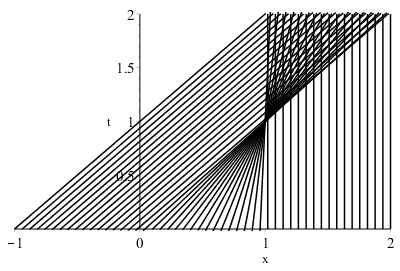
\includegraphics[width=0.5\linewidth]{./lect2/p2.png}
\end{center}

In point $x,y$ we have slope $u(x,y)$ thus the charecteristic curve crosses $x$-axis at $x_0 = x-uy$ and from initial conditions, $u=1-\frac{x_0}{\alpha}$. Thus
$$u=1-\frac{x-uy}{\alpha}$$
$$\alpha u=\alpha-x+uy$$
$$(\alpha-y) u=\alpha-x$$
Acquiring
$$u = \frac{x-\alpha}{y-\alpha}$$
And now for $y>1$ from Rankine–Hugoniot conditions
$$u(x,y) = \begin{cases}
1 & x<\alpha + \frac{1}{2} (y-\alpha)\\
0 & x>\alpha + \frac{1}{2} (y-\alpha)\\
\end{cases}$$
Such a solution is called a shock wave.

\begin{center}
	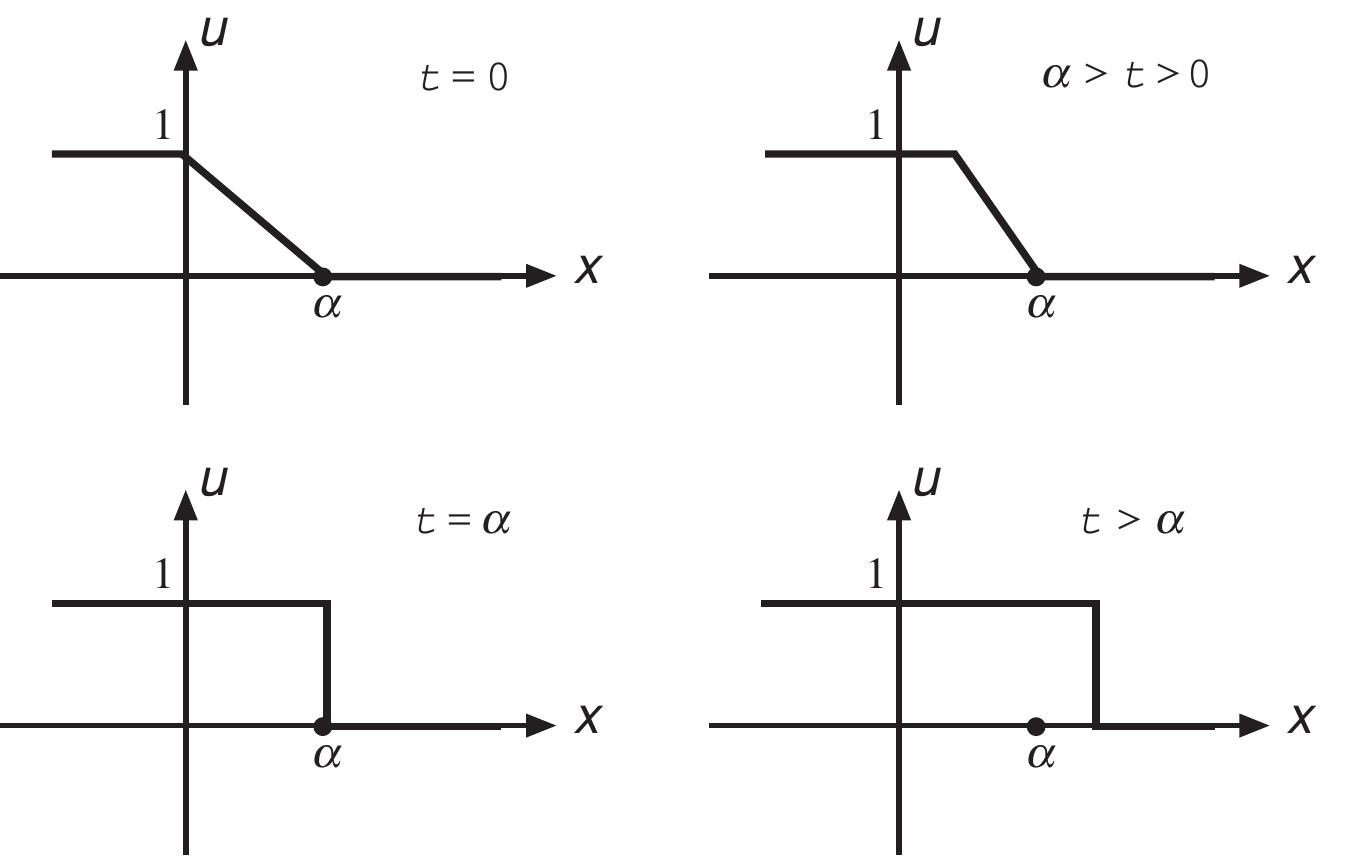
\includegraphics[width=0.7\linewidth]{./lect2/p1.png}
\end{center}

\paragraph{Example}
For
$$h(x) = \begin{cases}
0 & x> \alpha\\
1 & x < 0\\
\frac{x}{\alpha} & 0\leq x \leq \alpha
\end{cases}$$

Now there is no place where characteristic curves meet

\begin{center}
	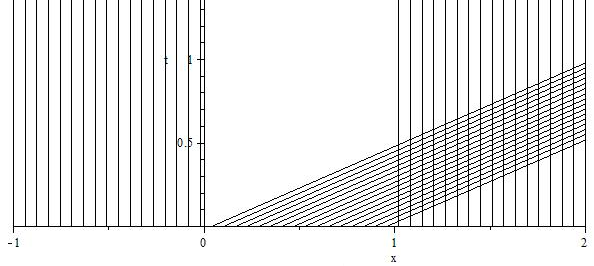
\includegraphics[width=0.7\linewidth]{./lect2/p3.png}
\end{center}

In the region without characteristic curves ($0\leq x\leq y$) we get the following: the solution starts from some  point $x_0 = x-uy$, and similarly to the previous case, from initial conditions,
$$u=\frac{x}{\alpha +y}$$


\begin{center}
	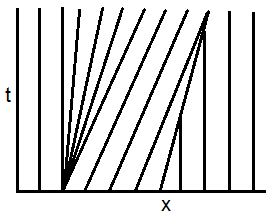
\includegraphics[width=0.3\linewidth]{./lect2/p4.png}
\end{center}

\paragraph{What happens if $\alpha \to 0$?}
We get $u=\frac{x}{y}$ for $0\leq x \leq y$. We acquired rarefaction wave - starting from something non-continuous we got continuous solution. This is weak solution.

However, also shock wave along $y=x$ is also solution of initial conditions. This solution is worse, because shock wave loses information, which means we cant reproduce the solution for some $y<y_0$ even if I know the values for $y=y_0$.
\paragraph{Entory principle}
Weak solution is unique if characteristic curves meet shock wave from direction of increasing time. 


\subsection{Fully non-linear equations}
\paragraph{Hamilton-Jacoby equation}
$$u_x^2+u_y^2=1$$
Can we generalize the method of solution of quasilinear equations to fully non-linear equations? The answer is yes. 
We have some $$F(x,y,u,u_x,u_y) = 0$$. In our case $$F(x,y,u,p,q) = p^2+q^2-1$$

Characteristic equations:
$$\begin{cases}
\dv{x}{t} = \pdv{F}{p}\\
\dv{y}{t} = \pdv{F}{q}\\
\dv{z}{t} = p\pdv{F}{p}+q\pdv{F}{q}\\
\dv{p}{t} = -\pdv{F}{x}+p\pdv{F}{z}\\
\dv{q}{t} = -\pdv{F}{y}+q\pdv{F}{z}\\
\end{cases}$$


Suppose we have initial curve $\Gamma = (\bar{x}(s), \bar{y}(s), \bar{z}(s))$

We need to find $\bar{p}$ and $\bar{q}$. We have two additional conditions:
$$F(x,y,u,u_x,u_y) = 0$$
also
$$u(\bar{x}(s), \bar{y}(s)) = \bar{z}(s)$$
Differentiating by $s$
$$\pdv{u}{x}\dv{\bar{x}}{s}  + \pdv{u}{y}\dv{\bar{y}}{s} = \dv{\bar{z}}{s}$$
$$\bar{p}(s)\dv{\bar{x}}{s} + \bar{q}(s)\dv{\bar{y}}{s} = \dv{\bar{z}}{s}$$
Now we can find $p$ and $q$.

Back to our equation:
$$\begin{cases}
\dot{x} = 2p\\
\dot{y} = 2q\\
\dot{z} = 2(p^2+q^2)\\
\dot{p} = \dot{q} = 0
\end{cases}$$

In case we have initial curve with $u=0$, then characteristic curves are perpendicular to initial curve.  We get $u(x,y)$ equal to distance from initial curve, since absolute value of gradient of $u$ is $1$ due to equation.

If we have $u=\phi(s)$ on initial curve, we acquire
$$u(x,y) = \min (x-\bar{x}(s))^2 + (y-\bar{y}(s))^2 + \phi(s)$$

\paragraph{Higher dimension}
We can trivially extend quasilinear equations to more dimensions. In this case we have initial surface instead of curve.
\section{Wave equation}
$$u_{tt} -c^2u_{xx} = 0$$
More generally, any second order linear equation can be written as
$$a(x,y) u_{xx} + 2b(x,y) u_{xy} + c(x,y) u_{yy} + du_x + eu_y + fu = g$$

\paragraph{Definition}
Equation is called hyperbolic if $b^2-ac>0$, parabolic if  $b^2-ac=0$ and elliptic if  $b^2-ac<0$. Wave equation is hyperbolic in the whole space.

We want to simplify the equation: we are searching for $\xi(x,y)$ and $\eta(x,y)$ such that
$$\pdv{\eta}{x} \pdv{\xi}{y} - \pdv{\eta}{y} \pdv{\xi}{x} \neq 0$$
and solution $u(x,y) = w\big(\xi(x,y), \eta(x,y)\big)$.

Derivatives of $u$ are
$$u_y = w_\xi \xi_y + w_\eta \eta_y$$
$$u_{yy} = w_{\xi\xi} \xi_{y}^2 + w_{\xi\eta}\xi_y\eta_y + w_{\xi}\xi_{yy} + w_{\eta \xi}\eta_y\xi_y + w_{\eta\eta} \eta_{y}^2+ w_{\eta}\eta_{yy}  $$
$$u_{xy} =\pdv{x}\pdv{u}{y} = w_{\xi \xi} \xi_x\xi_y + w_{\xi\eta}\xi_y\eta_x + w_{\xi\eta}\xi_x\eta_y + w_{\eta \xi} \eta_x\eta_y + w_{\xi}\xi_{xy}+w_\eta\eta_{xy}$$

Now we can get equation of form
$$A(\xi,\eta) w_{\xi\xi} + 2B(\xi,\eta) w_{\xi\eta} + C(\xi,\eta) w_{\eta \xi} + D(\xi,\eta) w_{\eta\eta}+ F(\xi,\eta) = 0$$
If we can find variable substitution such that
$$A=C=0$$
Then, in case of $d=e=f=0$,
$$Bw_{\xi\eta} = 0$$
i.e.,
$$w(\xi,\eta) = f(\xi)+g(\eta)$$
If we substitute derivatives back into general equation
\begin{align*}
au_{xx} + 2bu_{xy} + cu_{yy} = a \qty[w_{\xi\xi} \xi_{x}^2 + w_{\xi\eta}\xi_x\eta_x + w_{\xi}\xi_{xx} + w_{\eta \xi}\eta_x\xi_x + w_{\eta\eta} \eta_{x}^2+ w_{\eta}\eta_{xx} ] +\\+
2b\qty[w_{\xi \xi} \xi_x\xi_y + w_{\xi\eta}\xi_y\eta_x + w_{\xi\eta}\xi_x\eta_y + w_{\eta \xi} \eta_x\eta_y + w_{\xi}\xi_{xy}+w_\eta\eta_{xy}] +\\+ 
c\qty[w_{\xi\xi} \xi_{y}^2 + w_{\xi\eta}\xi_y\eta_y + w_{\xi}\xi_{yy} + w_{\eta \xi}\eta_y\xi_y + w_{\eta\eta} \eta_{y}^2+ w_{\eta}\eta_{yy} ]  =\\=
\qty\bigg(a\xi_x^2+3b\xi_x\xi_y + c\xi_y^2)w_{\xi\xi} + 2\qty\bigg(a\xi_x\eta_x + c\eta_y\xi_y + b(\xi_x\eta_y + \xi_y\eta_x))w_{\xi\eta} + \qty\bigg(a\eta_x^2+3b\eta_x\eta_y + c\eta_y^2)w_{\eta\eta} + \dots
\end{align*}
We can rewrite it in matrix form as
$$\begin{pmatrix}
\xi_x& \xi_y \\ \eta_x & \eta_y
\end{pmatrix} \begin{pmatrix}
a&b\\b&c
\end{pmatrix} \begin{pmatrix}
\xi_x& \eta_x\\ \xi_y  & \eta_y
\end{pmatrix} = \begin{pmatrix}
A&B\\B&C
\end{pmatrix}$$
$$\begin{vmatrix}
A&B\\B&C
\end{vmatrix} = \begin{vmatrix}
a&b\\b&c
\end{vmatrix} \cdot \begin{vmatrix}
\xi_x& \eta_x\\ \xi_y  & \eta_y
\end{vmatrix}^2$$
Since the determinant is exactly $ac-b^2$, under the variable substitution the sign of $b^2-ac$ is conserved.

\paragraph{Canonical form}
The form $w_{\xi \eta} + \ell_1[w] = G(\xi, \eta)$, where $\ell_1$ is first-order differential operator is called canonical form of hyperbolic equation.
\paragraph{Theorem} Each hyperbolic equation can be written in canonical form
\subparagraph{Proof}
We want to show that 
$$\begin{cases}
A = a\xi_x^2 + 2b\xi_x\xi_y + c\xi_y^2 = 0\\
C =a\eta_x^2 + 2b\eta_x\eta_y + c\eta_y^2 = 0
\end{cases}$$
i.e., that equation $a\psi_x^2 + 2b\psi_x\psi_y + c\psi_y^2 = 0$ has two independent solutions.

Dividing by $\psi_y^2$:
$$a\left(\frac{\psi_x}{\psi_y}\right)^2 + 2b\frac{\psi_x}{\psi_y} + c = 0$$
This is algebric equation, with solutions
$$\frac{\psi_x}{\psi_y} = \frac{-b\pm \sqrt{b^2-ac}}{a} = \lambda_\pm$$
We acquired a pair of equations
$$\psi_x - \lambda_\pm \psi_y = 0$$
And those are two independent solutions which result in $A=0$ and $C=0$.

\paragraph{Wave equation canonical form}
$$
u_{tt} - c^2 u_{xx} = 0$$
The canonical change of coordinates is
$$\begin{cases}
\xi = x-ct\\
\eta = x+ct
\end{cases}$$
$$u_{t} = -cw_\xi + cw_\eta$$
$$u_{x} = w_\xi + w_\eta$$
$$u_{tt} = c^2 w_{\xi\xi} - 2c^2w_{\xi\eta} +  c^2w_{\eta\eta}$$
$$u_{xx} = w_{\xi\xi} + 2w_{\xi\eta} + w_{\eta\eta}$$
Then
$$u_{tt} - c^2u_{xx} = -4c^2w_{\xi\eta}$$

The solution of canonical equation $w_{\xi \eta} = 0$ is $w(\xi, \eta) = F(\xi) + G(\eta)$, thus solution of wave equation:
$$u(x,t) = F(x+ct) + G(x-ct)$$

An example for physical object fulfilling wave equation is infinite string. To find a solution we need initial conditions, for example, velocity and location at time $t=0$:
$$\begin{cases}
u(x,0) = f(x)\\u_t(x,0) = g(x)
\end{cases}$$
, where $f\in \mathcal{C}^2$, $g\in \mathcal{C}^1$.
\paragraph{Theorem}
Exists unique solution of wave equation with those initial conditions. 
\subparagraph{Proof}
Substituting initial conditions into general solutions:
$$\begin{cases}
u(x,0) = F(x) + G(x) = f(x)\\
u_t(x,0) = c\qty[F'(x) - G'(x) ] = g(x)
\end{cases}$$
$$\begin{cases}
F'(x) + G'(x) = f'(x)\\
F'(x) - G'(x)  = \frac{g(x)}{c}
\end{cases} \Rightarrow \begin{cases}
F'(x) = \frac{f'(x) }{2} + \frac{g(x)}{2c}\\
G'(x)  = \frac{f'(x) }{2} - \frac{g(x)}{2c}
\end{cases} \Rightarrow \begin{cases}
F(x) = \frac{f(x) }{2} + \frac{1}{2c}\int_0^x g(s) \dd{s} + D_1\\
G(x)  = \frac{f(x) }{2} - \frac{1}{2c}\int_0^x g(s) \dd{s} + D_2
\end{cases}$$
Now, since $F(x)+G(x) = f(x)$, thus $D_1 + D_2 = 0$.

Substituting into solution, we acquire what is called d'Alembert's formula:
$$u(x,t) = \frac{f(x-ct) + f(x+ct) }{2} + \frac{1}{2c}\int_{x-ct}^{x+ct} g(s) \dd{s} $$
From construction, the solution is unique.
\paragraph{Example}
$$\begin{cases}
g(x) = 0 \\
f(x) = e^{-x^2}
\end{cases}$$
$$u(x,t) = \frac{1}{2} e^{-(x+ct)^2} + \frac{1}{2}e^{-(x+ct)^2} $$
\paragraph{Standing wave}
To get standing wave we want $G=0$, i.e., 
$$\begin{cases}
f(x) = F(x)\\
g(x) = cF'(x)
\end{cases} \Rightarrow g(x) = cf'(x)$$
\paragraph{Domain of dependence and region of influence}
Domain of dependence of $u$ in point $(x_0,t_0)$ is a characteristic triangle with vertices $(x_0-ct_0,0)$, $(x_0+ct_0, 0)$, $(x_0,t_0)$. Any point outside of triangle doesn't affect the value of $u$ in point.

Region of influence of point $x_0$ is cone bounded by condition $x_0-ct<x<x_0+ct$.
\begin{center}	
	\includesvg[eps,svgpath = lect3/,width=0.5\linewidth]{pic1}
\end{center}
%TODO
\paragraph{Weak solution}
$$\begin{cases}
g(x) = 0\\f(x) = \begin{cases}
1 & |x| <1 \\
0 & |x| > 1
\end{cases}
\end{cases}$$
The weak solution
$$u(x,t) = \frac{1}{2}f(x-ct)+\frac{1}{2}f(x+ct)$$
is not differentiable, but is solves the equation in some sense.
\subsection{Generalization of  d'Alembert's formula for non-homogeneous equations}
Consider non-homogeneous equation
$$u_{tt} - c^2 u_{xx} = \varphi(x,t)$$

Remember Green's theorem, for differentiable $P$ and $Q$ defined in $\Omega$:
$$\iint\limits_\Omega \pdv{Q}{x} - \pdv{Q}{t} \dd{x} \dd{t} = \oint\limits_{\partial \Omega} P(x,t) \dd{x} + Q(x,t) \dd{t}$$

Lets define $Q=c^2u_x$ and $P=u_t$, and choose $\Omega(x_0, t_0)$ to be characteristic triangle.

$$\iint\limits_{\Omega(x_0, t_0)} \varphi(x,t) \dd{x} \dd{t} = \iint\limits_{\Omega(x_0, t_0)} u_{tt} - c^2 u_{xx} \dd{x} \dd{t} = \oint P(x,t) \dd{x} - Q(x,t) \dd{t} = - \qty[\oint\limits_{\partial \Omega(x_0, t_0)} u_t \dd{x} + c^2u_x \dd{t}] $$

Lets divide the curve integral into three integrals along each of lines. For first line $\dd{t} = 0$, for second $\dd{x} + c\dd{t} = 0$ and for third $\dd{x} - c\dd{t} = 0$.
\begin{align*}
\oint\limits_{\partial \Omega(x_0, t_0)} u_t \dd{x} + c^2u_x \dd{t} =\\= \int_{x_0-ct_0}^{x_0+ct_0} \underbrace{u_t}_{g(x) \text{ in } t=0} \dd{x} - \int_{(x_0+ct_0,0)}^{(x_0, t_0)} cu_t \dd{t} + u_x \dd{x} +  \int_{(x_0, t_0)}^{(x_0-ct_0,0)} cu_t \dd{t} + u_x \dd{x} =\\= \int_{x_0-ct_0}^{x_0+ct_0} g(s) \dd{s} - c\int_{(x_0+ct_0,0)}^{(x_0, t_0)} \dd{u} + c \int_{(x_0, t_0)}^{(x_0-ct_0,0)} \dd{u} 
\end{align*}
Since
$$\int_{(x_0+ct_0,0)}^{(x_0, t_0)} \dd{u} = u(x_0, t_0) - f(x_0+ct_0) $$
$$ \int_{(x_0, t_0)}^{(x_0-ct_0,0)} \dd{u} = f(x_0-ct_0) -  u(x_0, t_0) $$
we get
$$\iint\limits_{\Omega(x_0, t_0)} \varphi(x,t) \dd{x} \dd{t} = -\int_{x_0-ct_0}^{x_0+ct_0} g(s) \dd{s} + 2cu(x_0, t_0) - cf(x_0+ct_0) - cf(x_0-ct_0) $$
from which we get the solution

$$u(x,t) = \frac{f(x-ct) + f(x+ct) }{2} + \frac{1}{2c}\int_{x-ct}^{x+ct} g(s) \dd{s} + \frac{1}{2c}\iint\limits_{\Omega(x_0, t_0)} \varphi(\xi, \eta) \dd{\xi} \dd{\eta}$$

We've got a cadidate for the solution. Let's check that $u$ is actually solving PDE. Define $v$, $w$, such that $w$ is a solution of homogeneous PDE and $v=u-w$, i.e.,
$$v(x,t) = \frac{1}{2c}\iint\limits_{\Omega(x_0, t_0)} \varphi(\xi, \eta) \dd{\xi} \dd{\eta}$$

Let's show that $v$ solves PDE. Rewrite $v$ as double integral:
$$v(x,t) = \frac{1}{2c}\int_0^t \int_{x-c(t-\tau)}^{x+c(t-\tau)} \varphi(\xi, \tau) \dd{\xi} \dd{\tau}$$
Define
$$H(x,t,\tau) = \int_{x-c(t-\tau)}^{x+c(t-\tau)} \varphi(\xi, \tau) \dd{\xi}$$
and then
$$v(x,t) = \frac{1}{2c} \int_0^t H(x,t,\tau) \dd{\tau}$$
$$\pdv{v}{t} = \frac{1}{2c} \underbrace{H(x,t,t)}_{0} +\frac{1}{2c} \int_0^t \pdv{H}{t}(x,t,\tau) \dd{\tau}$$
$$\pdv{H}{t} =c[\varphi(x+c(t-\tau), \tau) + \varphi(x-c(t-\tau), \tau) ]$$
$$\pdv[2]{H}{t} =c^2[\varphi_x(x+c(t-\tau), \tau) - \varphi_x(x-c(t-\tau), \tau) ]$$
$$\pdv[2]{v}{t} =\frac{1}{2c} \int_0^t \pdv[2]{H}{t}(x,t,\tau) \dd{\tau} =  \varphi(x,t) + \frac{c}{2} \int_0^t \varphi_x(x+c(t-\tau), \tau) - \varphi_x(x-c(t-\tau), \tau)  \dd{\tau} $$
$$\pdv{v}{x} = \frac{1}{2c} \int_0^t \pdv{H}{x} \dd{\tau}$$
$$\pdv{H}{x} = \varphi(x+c(t-\tau),\tau) - \varphi(x-c(t-\tau),\tau)$$
$$\pdv[2]{H}{x} = \varphi_x(x+c(t-\tau),\tau) - \varphi_x(x-c(t-\tau),\tau)$$
$$\pdv[2]{v}{x} = \frac{1}{2c} \int_0^t \varphi_x(x+c(t-\tau),\tau) - \varphi_x(x-c(t-\tau),\tau) \dd{\tau}$$
Thus we got
$$\pdv[2]{v}{t} - c^2\pdv[2]{v}{x} = \varphi(x,t)$$

Suppose we have two solutions $u_1$ and $u_2$ then $u=u_1-u_2$ is solution of homogeneous equation with $0$ initial conditions, and thus $u=0$. That means the solution is unique.

The presented initial condition problem has 3 properties:
\begin{enumerate}
	\item Solution exist
	\item It's unique
	\item It's stable
\end{enumerate}
\paragraph{Stability of wave equation}
For all $\tau > 0 $, $\epsilon >0$, exists $\delta >0$ such that if 
$$\begin{cases}
|f(x) - \tilde{f}(x) | < \delta\\
|g(x) - \tilde{g}(x) | < \delta\\
|\varphi(x) - \tilde{\varphi}(x) | < \delta\\
\end{cases}$$
For all $-\infty < x < \infty$ and $0 \leq t \leq \tau$ and if $u$, $\tilde{u}$ are solutions of corresponding wave equations, then
$$|u(x,t) - \tilde{u}(x,t)| < \epsilon$$
\subparagraph{Proof}
From the general solution:
\begin{align*}
u(x,t) - \tilde{u}(x,t) =\\= \qty|\frac{f(x+ct) + f(x-ct)}{2} - \frac{\tilde{f}(x+ct) + \tilde{f}(x-ct)}{2} + \frac{1}{2c}\int_{x-ct}^{x+ct} g(s) - \tilde{g}(s)\dd{s}  + \frac{1}{2c}\iint\limits_{\Omega(x_0, t_0)} \varphi(\xi, \eta) - \tilde{\varphi}(\xi, \eta)\dd{\xi} \dd{\eta}| \leq\\\leq \qty|\frac{f(x+ct) - \tilde{f}(x+ct)}{2}| + \qty|\frac{f(x-ct) - \tilde{f}(x-ct)}{2}| + \frac{1}{2c}\int_{x-ct}^{x+ct} \qty|g(s) - \tilde{g}(s)|\dd{s}  + \frac{1}{2c}\iint\limits_{\Omega(x_0, t_0)} \qty|\varphi(\xi, \eta) - \tilde{\varphi}(\xi, \eta)|\dd{\xi} \dd{\eta} \leq\\\leq \frac{\delta}{2}+\frac{\delta}{2} \frac{1}{2c} \cdot 2c \cdot \delta + \frac{1}{2c} \frac{ct}{2} = 2\delta + \frac{\delta t}{4} \leq 2\delta + \frac{\delta \tau}{4} \leq \epsilon
\end{align*}
Thus we choose $\delta < \frac{\epsilon}{2+\frac{\tau}{4}}$.
\subsection{Wave equation with bound conditions}
\paragraph{Half-infinite string}
Suppose string is fixed in one of its ends, at $x=0$: $u(0,t) = 0$. This is called Dirichlet boundary condition. We want to solve the PDE for $x>0$.

\subparagraph{Property of wave equation}
If $u(x,t)$ is solution, then $u(-x,t)$ is also solution:
$$u(x,t) = F(x+ct) + G(x-ct)$$
$$u(-x,t) = F(-x+ct)+G(-x-xt) = \bar{F}(x+ct) + \bar{G}(x-ct)$$
Where $\bar{F}(s) = G(-s)$ and $\bar{G}(s) = F(-s)$.

Lets extend $f$ and $g$ on the whole plane in odd way:
$$\bar{f}(x) = \begin{cases}
f(x) & x>0\\
-f(x) & x<0
\end{cases}$$
and same for $g$. 

Note that initial conditions have to be consistent, i.e., $f(0)=0$, $g(0)=0$, else the solution is discontinuous in 0.
Lets use D'Lambert solution:
$$\bar{u}(x,t) = \frac{\bar{f}(x+ct) + \bar{f}(x-ct)}{2} + \frac{1}{2c} \int_{x-ct}^{x+ct} \bar{g}(s) \dd{s}$$
Then the solution of half-infinite string is
$$u(x,t) = \begin{cases}
\frac{f(x+ct) + f(x-ct)}{2} + \frac{1}{2c} \int_{x-ct}^{x+ct} g(s) \dd{s}& x>ct\\
\frac{f(x+ct) - f(ct-x)}{2} + \frac{1}{2c} \int_{ct-x}^{x+ct} g(s) \dd{s}& x<ct\\
\end{cases}$$ 
\paragraph{Neumann boundary condition}
In this case, instead of giving boundary condition on $u$, we give boundary condition of $u_x$: $u_x(0,t) = 0$. Physical meaning is that there is no force in this point. In this case we will extend function in even way (derivative of even function in 0 is 0). Then we get$$u(x,t) = \begin{cases}
\frac{f(x+ct) + f(x-ct)}{2} + \frac{1}{2c} \int_{x-ct}^{x+ct} g(s) \dd{s}& x>ct\\
\frac{f(x+ct) + f(ct-x)}{2} + \frac{1}{c} \int_{0}^{ct-x} g(s) \dd{s} + \frac{1}{2c} \int_{ct-x}^{x+ct} g(s) \dd{s}& x<ct\\
\end{cases}$$ 
\paragraph{Uniquness}
Suppose we have two solutions, by subtracting them, we get
$$\begin{cases}
u_{tt} -c^2u_{xx} = 0\\u(x,0) = u_x(x,0) = 0\\ u(0,t) = 0
\end{cases}$$
We acquire $u(x,t)=0$. Since $u(x,t)$ is of form $F(x+ct)+G(x-ct)$, we get that twobsolutions are identical.
\paragraph{Wave equation with finite string}
Suppose we have string from $a$ to $b$:
$$\begin{cases}
u_{tt} - c^2u_{xx} = 0 & a\leq x \leq b \\
u(x,0) = f(x) \\
u_t(a,t) = h(t)\\
u_t(b,t)b= q(t)\\
\end{cases}$$
Here the consistency conditions are
$$\begin{cases}
h(0) = f(a) & q(0) = f(b)\\
h'(0) = g(a) & q'(0) = g(b)
\end{cases}$$
Here we could have conditions derivatives instead of values as well.
\paragraph{Parallelogram identity}

\begin{center}
	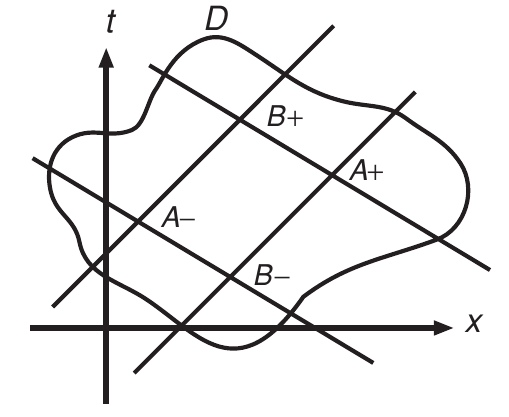
\includegraphics[width=0.4\linewidth]{./lect4/pic1.png}
\end{center}
$u\in \mathcal{C}^2$ is the solution of wave equation iff for any parallelogram with sides parallel to characteristic lines with vertices $A_-$, $A_+$, $B_-$, $B_+$ 
$$u(A_-)+u(A_+) = u(B_-) + u(B_+)$$
\subparagraph{Proof}
One direction is simple, since value of solution is constant along characteristic curves.

For second direction lets switch to canonical coordinates
$$\begin{cases}
\xi = x+ct\\
\eta = x-ct
\end{cases}$$
So
$$w(\xi, \eta) = u\qty(\frac{\xi+\eta}{2} ,\frac{\xi-\eta}{2})$$
$w$ is solution of wave equation iff $w_{\xi \eta} = 0$. 

Note that parallelogram turned into rectangular in new coordinates, i.e.,
$$w(\xi_0, \eta_1) + w(\xi_1, \eta_0) = w(\xi_1, \eta_1) + w(xi_0, \eta_0)$$
Dividing by $(\xi_1-\xi_0)(\eta_1-\eta_0)$:
$$\frac{w(\xi_0, \eta_1) + w(\xi_1, \eta_0) }{(\xi_1-\xi_0)(\eta_1-\eta_0)} - \frac{w(\xi_1, \eta_1) + w(xi_0, \eta_0)}{(\xi_1-\xi_0)(\eta_1-\eta_0)} = 0$$
Taking limit:
$$\lim_{\xi_1\to \xi_0} \lim_{\eta_1\to \eta_0} \frac{w(\xi_0, \eta_1) + w(\xi_1, \eta_0) - w(\xi_1, \eta_1) -  w(xi_0, \eta_0)}{(\xi_1-\xi_0)(\eta_1-\eta_0)} = w_{\xi\eta} = 0$$


In this way we can solve wave equation on finite range:
\begin{center}
	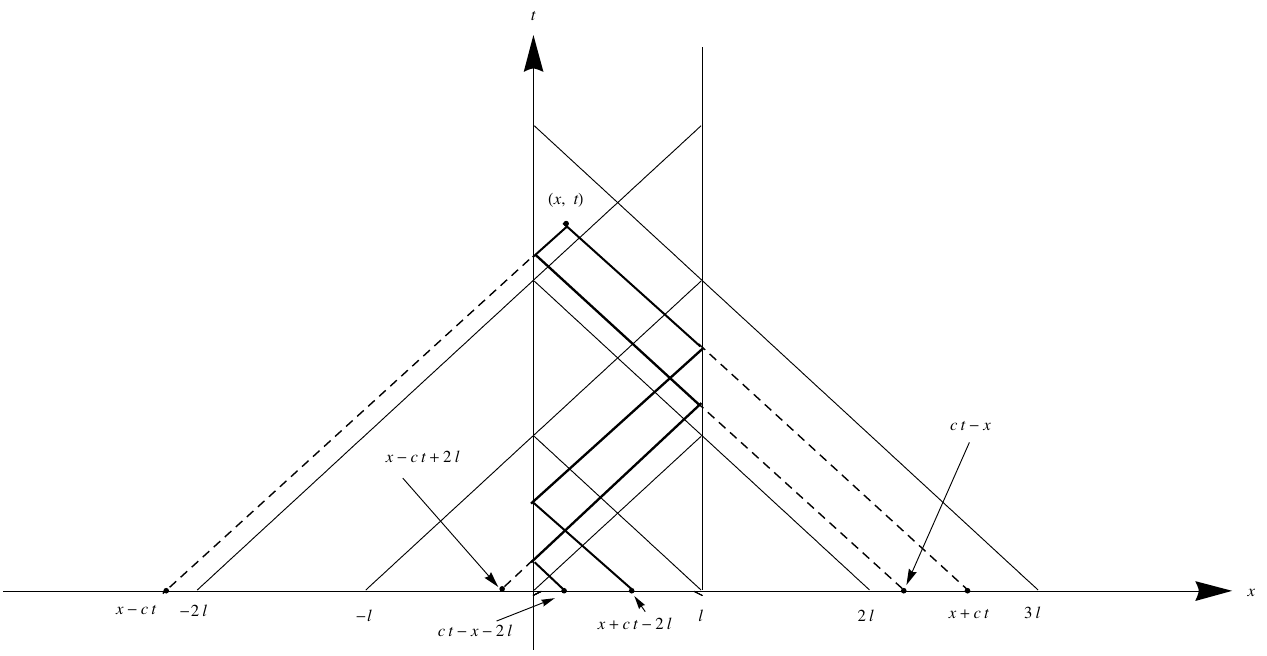
\includegraphics[width=\linewidth]{./lect4/pic2.png}
\end{center}
Using this method we can get solution for homogeneous wave equation for finite string.
\paragraph{Non-homogeneous wave equation}
$$u_{tt} -c^2u_{xx} = \varphi(x,t)$$
In this case parallelogram identity doesn't work. 

Lets extend $\varphi$ to the half plane $x>0$ to some function $\tilde{\varphi} \in \mathcal{C}^1$.


Lets solve non-homogeneous equation with 0  initial conditions:
 $w= \frac{1}{2c}\int\limits_{\triangle} \tilde{\varphi}$.


 with D'Lambert formula. 
 Lets solve homogeneous equation in the interval:
 $$\begin{cases}
 v(a,t) = h(t) + w(a,t)\\
 v(b,t) = q(t)+ w(b,t)\\
 v(x,0) = f(x)\\
 v_t(x,0) = g(x)
 \end{cases}$$
 
 Then the solution is
 $$u(x,t)= w(x,t)+v(x,t)$$
Checking the solution:
$$u_{tt} - c^2u_{xx}=  w_{tt} - c^2w_{xx} + v_{tt} - c^2v_{xx} = \tilde{\varphi}(x,t)  $$
which is $\varphi(x,t)$ in our interval.
\paragraph{Energy method}
Define
$$E(t) = \int_a^b \qty[ u_t^2(x,t) + c^2u_x^2(x,t)] \dd{x}$$ 
If $u\in \mathcal{C}^2$ we can differentiate it:
$$\dv{E}{t} = \int_a^b \qty[2u_tu_{tt} + 2c^2u_xu_{xt}] \dd{x} = 2c^2\int_a^b \qty[u_t u_{xx} + u_xu_{xt}]\dd{x} = 2c^2 \int_a^b (u_xu_t)_x \dd{x} = 2c^2 \qty[u_x(b,t)u_t(b,t) - u_x(a,t) u_t(a,t)]$$
If any combination of Dirichlet and Neumann conditions is fulfilled, the integral is $0$, i.e., energy is conserved. Thus
$$E(t) = E(0) = \int_a^b g^2(x) + c^2\qty(f'(x))^2 \dd{x}$$

From that we can conclude the solution is unique. As usual, suppose there are two solutions, $u$ and $v$. Subtracting we get a solution for homogeneous equation with homogeneous initial conditions $w=u-v$. Then $E_w(t) = E_w(0)=0$, thus $w_x=w_t=0$ and $w(x,t)=0$.

Also, from energy difference, we can conclude the solutions are stable.
\subsection{Variable separation}
Lets guess solution of form
$$U(x,t) = A(x)B(t)$$
Substituting into wave equation:
$$u_{tt} - c^2u_{xx} = A(x)B''(t) - c^2A''(x) B(t) = 0$$
Dividing by $A(x)B(t)$ (assume they are not zero):
$$\frac{B''(t)}{B(t)} = c^2\frac{A''(x)}{A(x)} = \mu$$
That means
$$\begin{cases}
A'' = \frac{\mu}{c^2}A = -\lambda A \\
B'' = \mu B
\end{cases}$$

Back to initial conditions $u(0,t)=u(1,t)=0$, that means $A(0) =A(1) = 0$. The question is when
$$A''+\lambda A = 0 $$
If $\lambda< 0$, the solution is
$$A = \alpha e^{-\sqrt{-\lambda}x} + \beta e^{\sqrt{\lambda}x}$$
Substituting initial conditions we get
$$\begin{cases}
\alpha+\beta=0\\
\alpha e^{-\sqrt{-\lambda}} + \beta e^{\sqrt{-\lambda}} = 0
\end{cases}$$
Since $\lambda\neq 0$, we conclude $\alpha=\beta=0$ which is trivial solution.
If $\lambda=0$ we get $A=\alpha x+\beta$, which is also trivially $A=0$.
If $\lambda>0$,
$$A = \alpha \sin(\sqrt{\lambda}x)+ \beta\cos(\sqrt{\lambda}x)$$
Since $A(0) = 0$, $\beta=0$. Since $A(1) = 0$, $\sqrt{\lambda} = k\pi$ for some $k \in \mathbb{N}$, i.e., $\lambda_k = k^2\pi^2$. The solution is 
$$A_k = \sin(k\pi x)$$

Back to $B$:
$$\frac{B''}{B} = - c^2k^2\pi^2$$
i.e.,
$$B_k(t) = a_k\sin(ck\pi t)+b_k\cos(ck\pi t)$$
Thus the solution of wave equation
$$u_k(x,t) = a_k \sin(k\pi x)\sin(ck\pi t)+b_k \sin(k\pi x)\cos(ck\pi t)$$
(note, that by using trigonometric identities we can get it to canonical form).

Define 
$$u(x,t) \sim \sum_{k=1}^\infty  a_k \sin(k\pi x)\sin(ck\pi t)+b_k \sin(k\pi x)\cos(ck\pi t)$$
Substituting $t=0$:

$$u(x,0) = \sum_{k=1}^\infty b_k \sin(k\pi x) = f(x)$$
$$u_t(x,0) = c\pi \sum_{k=1}^\infty k a_k \sin(k\pi x)\ = g(x)$$

If we'll find $a_k$, $b_k$ fulfilling those conditions, then we have a ``solution''. How we find them? Look at following integral:
$$\int_0^1 f(x) \sin(n \pi x) \dd{x} = \int_0^1 \qty[\sum_{k=1}^\infty b_k \sin(k\pi x)]\sin(n \pi x) \dd{x} = \sum_{k=1}^\infty b_k\underbrace{ \int_0^1  \sin(k\pi x)\sin(n \pi x) \dd{x}}_{\frac{\delta_{nk}}{2}} = \frac{b_n}{2}$$
Thus,
$$b_n = 2\int_0^1 f(x) \sin(n \pi x) \dd{x}$$
Exactly in the same way we can get
$$a_n = \frac{2}{c\pi n} \int_0^1 g(x) \sin(n \pi x) \dd{x}$$
If $\sum |ka_k| < \infty$ and $\sum |b_k| < \infty$, our series converge uniformly. If also $\sum |k^2a_k| < \infty$ and $\sum |kb_k| < \infty$, then $u(x,t) \in \mathcal{C}^1$. Analogously, if $\sum |k^3a_k| < \infty$ and $\sum |k^2b_k| < \infty$, $u\in \mathcal{C}^2$.

Suppose $\max\limits_{(0,1)} |f|<M_0$, then 
$$|b_n| \leq 2 \int_0^1 \abs{f(x) \sin (n\pi x)}\dd{x} \leq 2M_0$$. 
Suppose also that $f\in \mathcal{C}^1$ and  $\max\limits_{(0,1)} |f'|<M_1$ then
$$b_n = -\frac{2}{n\pi} \int_0^1 f(x) \qty(\cos(n \pi x))'\dd{x}$$
Integrating by parts and using the fact $f(0)=f(1)=0$:
 $$b_n = \frac{2}{n \pi} \int_0^1 f'(x) \cos(n \pi x) \dd{x} \leq \frac{2}{n\pi}M_1$$
 
 To show that $b_n<\frac{B_2}{n^2}$, we need $f\in \mathcal{C}^2$,  $\max\limits_{(0,1)} |f''|<M_2$ and $f'(0)+f'(1)=0$. % TODO

In general, if $f\in \mathcal{C}^l$ and sum $f^{(l-1)}(0) + f^{(l-1)}(1) = 0$, we can bound $|b_n| < \frac{B_l}{n^l}$.

\paragraph{Generalization}
$$\begin{cases}
u_{tt} - c^2 u_{xx} = \varphi(x,t)\\
u(x,0)=f(x)\\
u_t(x,0) = g(0)\\
u(0,t) = h(t)\\
u(1,t)= q(t)
\end{cases}$$
Define $w(x,t)$ such that $w(0,t) = h(t)$ and $w(1,t)=q(t)$ and $v=u-w$. Then
$$v_{tt}-c^2v_{xx} = u_{tt} - c^2 u_{xx} - w_{tt} + c^2w_{xx} = \varphi(x,t)- w_{tt} + c^2w_{xx}  = \tilde{\varphi}(x,t)$$

Thus we can assume bound conditions are $0$, as soon as we can solve non-homogeneous equation.

$$v_{tt} - c^2v_{xx} = \tilde{\varphi}(x,t)$$
Guess solution
$$v(x,t) = \sum_{k=1}^\infty q_k(t) \sin(k\pi x)$$
Substituting:
$$\sum_{k=1}^\infty \qty(q_k''(t) + k^2c^2\pi^2q_k(t)) \sin(k\pi x) = \tilde{\varphi}(x,t)$$
Suppose we can expand $$\tilde{\varphi}(x,t) = \sum_{k=1}^\infty p_k(t)\sin(k \pi x)$$.
$$\int_0^1 \tilde{\varphi} \sin (n\pi x) \dd{x} = \sum_{k=1}^\infty p_k(t) \int_0^1 \sin(k \pi x)\sin (n\pi x) \dd{x} = \frac{p_n(t)}{2}$$
Thus
$$p_n(t) = 2\int_0^1 \tilde{\varphi} \sin (n\pi x) \dd{x} $$
By coefficient comparison:
$$q_k''(t) + k^2c^2\pi^2q_k(t) = 2\int_0^1 \tilde{\varphi} \sin (n\pi x) \dd{x}$$

Since we know that
$$\begin{cases}
v(x,0) = \sum_{k=1}^\infty q_k(0) \sin(k\pi x) = f(x)\\
v_t(x,0) = \sum_{k=1}^\infty q'_k(0) \sin(k\pi x) = g(x)\\
\end{cases}$$
i.e.,
$$q_k(0) = 2\int_0^1 f(x) \sin(k \pi x) \dd{x}$$
$$q'_k(0) = 2\int_0^1 g(x) \sin(k \pi x) \dd{x}$$

Meaning we can solve ODE, and get solution for wave equation.

\paragraph{Neumann bound conditions}
Once again guessing the solution
$$\begin{cases}
u(x,t) = A(x)B(t)\\
u(x,0) = f(x)\\
u_t(x,0)= g(x)\\
A'(0) = A'(1) = 0
\end{cases}$$
We get once again
$$A(x) = a\sin(\sqrt{\lambda}x)+b\cos(\sqrt{\lambda}x)$$
$$A'(x) = \sqrt{\lambda}a\cos(\sqrt{\lambda}x)-\sqrt{\lambda}b\sin(\sqrt{\lambda}x)$$
Substituting initial conditions:
$$A'(0) = \sqrt{\lambda}a \Rightarrow a= 0$$
$$A'(1) = \sqrt{\lambda}b\sin(\sqrt{\lambda}x)$$
Thus we get the same $\lambda_k= k \pi$, however the series contains cosines instead of sines:
$$A_k(x) = \cos(k \pi x)$$
and we can solve in a similar way.
\paragraph{Operator of hyperbolic equation}
We can define linear operator
$$L(u) = \qty(a\pdv[2]{x}+2b\pdv{}{x}{y} + c \pdv[2]{y} + d\pdv{x} + f\pdv{y} + g)$$
Then the equation is
$$L(u) = h$$
We can turn it into canonical form:
$$L'(u) = \qty(\pdv{}{\xi}{\eta}  + d'\pdv{x} + f'\pdv{y} + g') $$
\paragraph{Cauchy problem for hyperbolic equation}
Given a curve in space $\va{r}(s) = \qty\big(\bar{x}(s), \bar{y}(s))$, ge define initial conditions
$$\begin{cases}
u\qty\big(x(s),y(s)) = h(s)\\
u_x\qty\big(x(s),y(s)) = \varphi(s)\\
u_y\qty\big(x(s),y(s)) = \psi(s)\\
\end{cases}$$

However, since we need two conditions, there is consistency requirement on those functions:
$$\dv{h}{s} = u_x\qty\big(x(s),y(s)) \pdv{\bar{x}}{s} + u_y\qty\big(x(s),y(s)) \pdv{\bar{x}}{s} = = \varphi(s) \pdv{\bar{x}}{s} + \psi(s) \pdv{\bar{x}}{s}  $$

Suppose we have equation of form
$$\begin{cases}
au_{xx} + 2bu_{xy} + cu_{yy} = d\\
u_{xx} \dv{\bar{x}}{s} + u_{xy} \dv{\bar{y}}{s} = \dv{\varphi}{s}\\
u_{xy} \dv{\bar{x}}{s} + u_{yy} \dv{\bar{y}}{s} = \dv{\psi}{s}
\end{cases}$$

To have an opportunity to evaluate second derivatives, we need to find solution of this linear system, i.e., we need that
$$\begin{vmatrix}
a&2b&c\\\dv{\bar{x}}{s}& \dv{\bar{y}}{s}&0\\0 &\dv{\bar{x}}{s}& \dv{\bar{y}}{s}
\end{vmatrix} \neq 0$$
or
$$a\qty(\dv{\bar{y}}{s})^2 - 2b\dv{\bar{x}}{s}\dv{\bar{y}}{s} + c\qty(\dv{\bar{x}}{s})^2 \neq 0$$
meaning the direction of tangent line is not in direction of characteristic lines.

We can derive the system once again and thus find third-order derivatives, doing it up to infinity, we get all the partial derivative.
\paragraph{Cauchy–Kowalevski theorem}
If the coefficients and initial curve are analytic functions, then exists unique analytic solution. 

\section{Heat equation}
For some positive $k$
$$u_t - ku_{xx}  = 0$$
Temperature $u(x,t)$ fulfills heat equation.
\paragraph{Dirichlet bound conditions}
$$u(a,0) =  u(b,0) = 0$$
\paragraph{Neumann bound conditions}
The meaning of Neumann bound condition is that there is heat isolation in interval bounds:
$$u_x(a,t) = u_x(b,t) = 0$$
$$Q(t) = \int_a^b u(x,t) \dd{x} $$
$$\dv{Q}{t} = \int_a^b \pdv{Q}{t}(x,t) \dd{x} = k \int_a^b \pdv[2]{u}{x} (x,t) \dd{x} = k \qty[\pdv{u}{x} (,t) - \pdv{u}{x} (a,t)] = 0$$
Thus $Q(t)$ is constant. $$Q(t)=Q(0) = \int_a^b f(x) \dd{x}$$
\paragraph{Solution of heat equation}
Suppose, for Dirichlet bound condition, that solution is series of sines.
$$u(x,t) = \sum_{n=1}^\infty a_n(t) \sin(n\pi x)$$
$$\pdv{u}{t} = \sum_{n=1}^\infty a'_n(t) \sin(n\pi x)$$
$$\pdv[2]{u}{x} = \sum_{n=1}^\infty -(n\pi)^2 a_n(t) \sin(n \pi x)$$

Then we get
$$\pdv{u}{t} - k \pdv[2]{u}{x} = \sum_{n=1}^\infty \qty[a'_n(t) + k(n\pi)^2 a_n(t) ]\sin(n\pi x) = 0$$
Thus, by coefficient comparison
$$a'_n(t) + k(n\pi)^2 a_n(t)  = 0$$
$$a_n(t) = a_n(0) e^{-k(n\pi)^2t}$$
$$u(x,t) = \sum_{n=1}^\infty a_n(0) e^{-k(n\pi)^2t}\sin(n\pi x)$$
From initial conditions we can find $a_n(0)$:
$$u(x,0) = f(x) = \sum_{n=1}^\infty a_n(0)\sin(n\pi x)$$

Our series is infinite differentiable if $t>0$.

If $t=0$, we need 
$$\lim_{t \to 0^-} u(x,t) = f(x)$$

For $t<0$, coefficients diverge, and thus we can't find solutions for $t<0$. Physically we can see it from entropy grows.

\paragraph{Example}
$$
\begin{cases}
u_t-ku_{xx} = 0 \\
u(x,0)  = 1\\
u(0,t) = u(1,t) = 0 & t>0
\end{cases}
$$
We acquire
$$a_n = \frac{1}{2} \int_0^1 1 \cdot \sin(n\pi x) \dd{x}$$
$$\abs{a_n} \leq \int_0^1 \dd{x} = \frac{1}{2} $$
Thus
$$\abs{a_n} \leq \frac{1}{2}e^{-k(n\pi)^2 t}$$
Thus the series absolutely converges for $t>0$.

In limit $t\to \infty $, $a_n \to 0$, and thus $u(x,t) \to 0$.

\paragraph{Stability}
For each $\epsilon>0$ exists $\delta > 0$ such that if
$$\max\limits_{a\leq x\leq b} \abs{u(x,0)} < \delta$$ % TODO
then
$$\max\limits_{a\leq x\leq b} \abs{u(x,t)} < \epsilon$$
\subparagraph{Proof}
We'll proof the weaker version of the theorem, with condition that $\sum \abs{a_n} < \delta$.

% If $u(x,0) = \sum_{n=1}^\infty a_n \sin(n\pi x)$, $a_n(0) < \frac{\delta}{2}$.
Then coefficients of $u(x,t)$ are bounded by
$$a_n(t) \leq e^{-k(n\pi)^2 t}\frac{\delta}{2}$$
i.e.
$$\abs{u(x,t)} \leq \sum_{n=1}^\infty \abs{a_n} e^{-k(n\pi)^2 t} < \sum |a_n| <\delta$$
\section{Potential equation} 
$$u_{xx} + u_{yy} = 0$$
Bound conditions are
$$\begin{cases}
u(x,0) = f(x)\\
u_x(x,0) = g(x)
\end{cases}$$

By variable separation we get
$$u_n =A_n(x)B_n(y)$$
we know that
$$A_n(x) = \sin(n\pi x) $$
Since
$$(n\pi)^2 = \frac{A_n''}{A_n} = -\frac{B_n''}{B_n}$$
$$B_n(y) = \alpha_n \sinh (n\pi y) + \beta_n \cosh(n \pi y)$$

\paragraph{Stability}
Is potential equation stable? Suppose $\max |f(x)| < \delta$ and $\max |g(x)| < \delta$

No. For example
$$u(x,y) = \frac{1}{n^3}e^{(n\pi)^2 y}\sin (n\pi x)$$
Then
$$u(x,0) = \frac{\sin(n\pi x)}{n^2}$$
$$u_y(x,0) = \frac{\sin(n\pi x)}{n}$$
This doesn't fulfills stability condition 
$$\abs{u_n(x,y)}<\epsilon$$
for large enough $n$.
\paragraph{Laplace equation}
$$\laplacian{u} = 0$$
If $u$ fulfills $\laplacian{u} = 0$, it is called harmonic function.
\paragraph{Poisson equation}
$$\laplacian{u} = f$$
Where $f$ describes mass/charge distribution in space.
\paragraph{Elliptic PDEs}
For elliptic equation $b^2-4ac<0$.
In this case, we can get the canonical form
$$u_{\xi\xi} + u_{\eta\eta} + L_1(\xi, \eta) = f$$
where $L_1$ is first-order differential operator.
\subsection{Laplace equation}
$$\div{\grad{u}} = \laplacian{u} = 0$$
\paragraph{Gauss law}
For vector field $\va{w} \in \mathcal{C}^1(\Omega) \cap \mathcal{C}(\bar{\Omega}$ 
$$\iint\limits_{\Omega} \div{\va{w}} \dd[3]{x} =  \oiint\limits_{\partial \Omega} \va{w} \vdot \vu{n} \dd{s}$$

Thus
$$\iiint\limits_{\Omega} \laplacian{\va{u}} \dd[3]{x} = \oiint\limits_{\partial \Omega} \pdv{u}{n} \dd{s}$$
i.e., if function is harmonic,
$$\oiint\limits_{\partial \Omega}  \pdv{u}{n} \dd{s} = 0$$

\paragraph{Conclusion}
The equation $\laplacian{u} = f $ in $\Omega$ for $u$ fulfilling $\pdv{u}{n}  = g$ in each point of  $\partial \Omega$ there is no solution if
$$\iiint\limits_{\Omega} \neq \oiint\limits_{\partial \Omega} g \dd{s}$$
The necessary condition for solution of Neumann problem 
$$\iiint\limits_{\Omega} = \oiint\limits_{\partial \Omega} g \dd{s}$$

For Dirichlet problem, there is no such constraint.

\paragraph{Examples of harmonic functions}
In $n=1$, linear functions are harmonic.

In $n=2$, any real or imaginary part of analytic function is harmonic, e.g., $e^x \sin y$.
\paragraph{The mean value property of harmonic function}
If $u$ is harmonic in $\Omega$ which contains $B_R(x) = \left\{ y| |x-y|<R \right\}$
then
$$u(x) = \frac{1}{\abs{\partial B_R(x)}} \oint\limits_{\partial \Omega} u \dd{s} $$
and
$$u(x) = \frac{1}{\abs{ B_R(x)}} \int\limits_{\Omega} u(y) \dd[n]{y} $$
\subparagraph{Proof}
Suppose $x=0$.
Rewrite $y\in B_R(x) $ as $y=\rho\alpha$ for $\alpha= \frac{y}{\norm{y}}$ and $\rho = \norm{y}$.

For each $\rho\in [0,R]$:
$$\int\limits_{B_\rho(0)} \pdv{u}{n} (\rho\alpha) \dd{s_y}=\int\limits_{B_\rho(0)} \pdv{u}{n} (y) \dd{s_y} = \iint \laplacian{u} \dd[n]{x} = 0$$
With variable substitution $\dd{s_y} = \rho^{n-1}\dd{s_\alpha}$:
$$\int\limits_{B_\rho(0)} \pdv{u}{n} (\rho\alpha) \dd{s_y}=\int\limits_{B_\rho(0)} \pdv{u}{n} (\rho\alpha) \rho^{n-1} \dd{s_\alpha}=\rho^{n-1} \int\limits_{B_\rho(0)} \pdv{u}{\rho} (\rho\alpha)  \dd{s_\alpha} = \rho^{n-1}  \pdv{\rho} \int\limits_{B_\rho(0)}  u(\rho\alpha)  \dd{s_\alpha}$$
Thus
$$\pdv{\rho} \int\limits_{B_\rho(0)}  u(\rho\alpha)  \dd{s_\alpha} = 0$$
meaning
$$H(\rho) = \int\limits_{B_\rho(0)}  u(\rho\alpha)  \dd{s_\alpha} = \text{const}$$
Denote volume of unit ball as $\omega_n$, then $\abs{B_n} = \omega_n R^n$ and $\abs{\partial B_n} = \omega_{n-1}R^{n-1}$ 
$$H(0) = \omega_n \cdot u(0)$$
And since $H(1) = H(0)$:
$$u(0) = \frac{1}{n\omega_n R^{n-1}} \int\limits_{\partial B_R(0)} \dd{s}$$
as required.

$$\omega_n \rho^{n-1} u(0) = \int\limits_{\partial B_\rho(0)} u(y) \dd{s_y}$$
$$\int_0^R n \omega_n \rho^{n-1} u(0) \dd{\rho} = \int_0^R \dd{\rho} \int\limits_{\partial B_\rho(0)}  \dd{s_y} u(y)$$
$$\omega_n R^n u(0) = \iint\limits_{B_r(0)} u(y) \dd[n]{y}$$
i.e.,
$$u(0) = \frac{1}{\abs{B_r(0)}} \iint\limits_{B_r(0)} u(y) \dd[n]{y}$$
	\paragraph{Strong maximum principle }
	If $u$ is harmonic and it acquires maximum or minimum, then it is constant.
	\paragraph{Subharmonic and superharmonic functions}
	Subharmonic function is function for which $\laplacian{u}\leq 0$ and superharmonic is one for which $\laplacian{u}\geq0$.
	
	In this case, strong maximum principle applies only in one direction (maximum for subharmonic, minimum for superharmonic). For mean value theorem we get inequality instead of equality.
	
	\subparagraph{Proof}
	let $u$ subharmonic, and $m = u(x) = \max\limits_{\Omega} u$.
	The set $W= \left\{ y: u(y)=m \right\} $ is closed relatively to $\Omega$.
	Let $z\in W$, $B_R(z) \in \Omega$.
	$$m = u(z) \leq \frac{1}{\abs{B_R(z)}} \int\limits_{B_r(z)} \int u(y) \dd[n]{y} = m$$
	
	Thus for all $z\in W$
	$$u(z) = \frac{1}{\abs{B_R(z)}} \int\limits_{B_r(z)} \int u(y) \dd[n]{y}$$
	That means
	$$\int\limits_{B_r(z)} u(x) - m \dd[n]{x}= 0$$
	Thus $u(x) = m$ for all $x\in B_R(z)$, which turns $W$ is open set. Thus $W$ is both open and closed, i.e. $W=\Omega$.
	
	\paragraph{Conclusion}
	Poisson equation $\laplacian{u} = f$ in $\Omega$ with bound condition $u_{\partial \Omega} = y$ has not more than one solution.
	\subparagraph{Proof}
	Suppose there are two solutions, $u_1=u_2$, define $v=u_1-u_2$ is harmonic function with ound condition  $v_{\partial \Omega} = 0$. The function $v$ is harmonic. If $v\neq 0$, it has either maximum or minimum, in contradiction with strong maximum principle.
	
	\paragraph{Weak maximum principle}
	For compact connected $\Omega$ and $u = \mathcal{C}^2(\Omega) \cap \mathcal{C}(\partial \Omega)$ 
	
	If $\laplacian{u} \leq 0$, 
	$$\max\limits_{\bar{\Omega}} u = \max\limits_{\partial \Omega} u$$
	If $\laplacian{u} \geq 0$, 
	$$\min\limits_{\bar{\Omega}} u = \min\limits_{\partial \Omega} u$$
	\paragraph{Harnack's inequality}
	If $u$ harmonic and non-negative in interval $\Omega$ and $\bar{\Omega'} \subsetneq \Omega$, then exists constant $c(\Omega, \Omega')$ independent on $u$ such that
	$$\sup\limits_{\Omega'} u \leq c \inf\limits_{\Omega} u$$
	
i.e., for any two points $x,y \in \Omega'$
$$u(x) \leq cu(y)$$
\subparagraph{Proof}
Let $\Omega = B_{4R}(y)$ and $\Omega' = B_{R}(y)$. Choose $x_1, x_2 \in \Omega'$.

Since $B_R(x_1) \subset B_{4R}(y)$, we can use the mean value property:
$$u(x_1) = \frac{1}{\omega_n R^n } \int\limits_{B_R(x_1)} \dd{x} u \leq \frac{1}{\omega_n R^n } \int\limits_{B_{2R}(y)} \dd{x} u$$
Similarly, since $B_{3R}(x_1) \subset B_{4R}(y)$, we can use the mean value property:
$$u(x_2) = \frac{1}{\omega_n (3R)^n } \int\limits_{B_{3R}(x_2)} \dd{x} u \geq \frac{1}{\omega_n (3R)^n } \int\limits_{B_{2R}(y)} \dd{x} u = \frac{1}{3^n} \frac{1}{\omega_n R^n } \int\limits_{B_{2R}(y)} \dd{x} u \geq u(x_1)$$
We got
$$3^nu(x_2) \leq u(x_1)$$

Since $\bar{\Omega'} \subsetneq \Omega$, there exists $R>0$ such that distance from any point of $\Omega'$ to any point of $\Omega^c$ is greater than $4R$.

For any pair of points $x_1, x_2 \in \Omega$, the path between then can be covered by $m$ balls $B_j$ of radius $R$, such that intersection of each pair of consequentive balls is non-empty.

So, let $y_j \in B_j \cap B_{j+1}$ and $y_1=p$, $y_m=q$, then $u(y_j) \leq 3^n u(y_{j+1})$, since $y_j, y_{j+1} \in _{j+1}$ and $B_{4R}(y_{j+1}) \subset \Omega$.
Than means that
$$u(q) \leq 3^{nm} u(p)$$
\paragraph{Radial harmonic functions }
Lets search for harmonic functions of form $u(x)=f(r)$ for $f$ defined on $\mathbb{R}^+$.
$$\abs{x} = \sqrt{\sum x_i} = r$$
is harmonic on $\mathbb{R}^n \setminus 0$ and radial.
$$\pdv{r}{x_i} = \frac{x_i}{r}$$
$$\pdv[2]{r}{x_i} = \frac{1}{r} - \frac{x_i^2}{r^2}$$
Thus
$$\pdv{u}{x_i} = f'(r) \pdv{r}{x_i} = f'(r) \frac{x_i}{r}$$
$$\pdv[2]{u}{x_i} = f''(r) \qty(\frac{x_i}{r})^2 - f'(r) \qty(\frac{1}{r} - \frac{x_i^2}{r^2})$$
$$\laplacian{u} = f''(r) \sum \qty(\frac{x_i}{r})^2  - f'(r) \qty(\frac{n}{r} - \frac{\sum x_i^2}{r^2}) = f''(r) + \frac{n-1}{n}f'(r) = 0$$
This is Euler equation with solution
For $n=2$
$$f(r) = c_1 \ln r + c_2$$
For $n>2$:
$$f(r) = \frac{c_1}{r^{n-2}} + c_2$$
\paragraph{Fundamental solution}
Define fundamental solution of Laplace equation:
$$
\begin{cases}
\Gamma(r) = \frac{1}{2\pi} \ln(r)&n=2\\
\Gamma(r) = \frac{1}{n(2-n)\omega_n}r^{2-n}& n>2\\
\end{cases}$$
We conclude that $\Gamma(\abs{x-y})$ is harmonic function in $\mathbb{R}^n \setminus \{y\}$.

For $n=2$
$$\lim_{r\to \infty}\Gamma(n) = \infty $$
and for $n>2$
$$\lim_{r\to \infty}\Gamma(n) = 0 $$
Also, for any $n\geq 2$
$$\lim_{r\to 0} \Gamma(n) = -\infty$$

\paragraph{Homogenity of $\Gamma$}
For $n>2$
$$\pdv{\Gamma(x-y)}{x_i} = \frac{1}{n\omega_n} \frac{x_i-y_i}{\abs{ x-y}^n} $$

$$\pdv{\Gamma}{x_i}{x_j} = \frac{1}{n\omega_n} \qty[\abs{x-y}^2 \delta_{ij} - n(x_i-y_i)(x_j-y_j)] \abs{x-y}^{-n-2}$$
$$\abs{\pdv{\Gamma(x-y)}{x_i}} \leq \frac{1}{n\omega_n} \abs{x-y}^{1-n}$$
$$\abs{\pdv{\Gamma(x-y)}{x_i}{x_j}} \leq \frac{1}{n\omega_n} \abs{x-y}^{-n}$$
	Also
$$\begin{cases}
\Gamma'(r) = \frac{1}{n\omega_n r}& n=2\\
\Gamma'(r) = \frac{1}{n\omega_n} r^{1-n}
\end{cases}$$
\paragraph{Green identities}
If $\Omega \subset \mathbb{R}^n$ bounded set with boundcin $\mathcal{C}^2$ and
$u,v \in \mathcal{C}^2(\Omega) \cap \mathcal{C}^1(\bar{\Omega})$
$$\int\limits_{\Omega} v\laplacian{u} + \grad{u} \vdot \grad{v}  \dd{x} = \int\limits_{\partial \Omega} v \pdv{u}{n} \dd{s} $$
$$\int\limits_{\Omega} v\laplacian{u} - u \laplacian{v} \dd{x} = \int\limits_{\partial \Omega} v \pdv{u}{n} - u \pdv{v}{n} \dd{s} $$
\paragraph{}
If $\Omega \subset \mathbb{R}^n$ bounded set with bound in $\mathcal{C}^1$ and
$u \in \mathcal{C}^2(\Omega) \cap \mathcal{C}^1(\bar{\Omega})$
$$u(y) = \int\limits_{\Omega} \Gamma(x-y) \laplacian{u} \dd{x} + \int\limits_{\partial \Omega} \qty[u(x) \pdv{n_x}\Gamma(x-y) - \Gamma(x-y) \pdv{u}{n_x}] \dd{s_x} $$
If $u$ harmonic
$$u(y) =  \int\limits_{\partial \Omega} \qty[u(x) \pdv{n_x}\Gamma(x-y) - \Gamma(x-y) \pdv{u}{n_x}] \dd{s_x} $$

\subparagraph{Proof}
$\Gamma(x-y)$ is harmonic in $\Omega \setminus B_\rho(y) = \Omega_\delta$.
Choose $v(x) = \Gamma(x-y)$,
$$\int\limits_{\Omega_\delta} \Gamma\laplacian{u} \dd{x} = \int\limits_{\partial \Omega} \Gamma \pdv{u}{n} - u \pdv{\Gamma}{n} \dd{s_x} -  \int\limits_{\partial B_\rho(y)} \Gamma \pdv{u}{n} - u \pdv{\Gamma}{n} \dd{s} $$
Now
$$\int\limits{B_\rho(y)} \Gamma(\abs{x-y}) \laplacian{u(x)} \dd{x} \leq \max\limits_{B_\rho(y)} \cdot \int\limits{B_\rho(y)} \Gamma(\abs{x-y})  \dd{x} = \frac{\omega_n}{n\omega_n} \int_0^\rho r^{2-n}r^{n-1} \dd{r} = \frac{1}{n} \int_0^\rho  r \dd{r} = \frac{\rho^2}{2n} \stackrel{\rho\to 0}{\longrightarrow} 0 $$
$$\abs{\pdv{u}{n}} = \abs{\laplacian{u} \cdot n} \leq C $$
$$\abs{ \int\limits_{\partial B_\rho(y)} \Gamma \pdv{u}{n}} \leq C \int\limits_{B_\rho(y)} \abs{\Gamma} = \frac{c}{n\omega_n} \rho^{2-n} n\omega_n \rho^{n-1} =C \rho \to 0$$
$$\int\limits_{B_\rho(y)} u \pdv{\Gamma}{n} \dd{s_x} = \Gamma'(\rho)\int\limits_{B_\rho(y)} u \dd{s_x} = \frac{1}{n\omega_n \rho^{n-1}} \int\limits_{B_\rho(y)} u \dd{s_x}\stackrel{\rho\to 0}{\longrightarrow} u(y) $$

Substituting it back into equation we get exactly what was needed:
$$u(y) = \int\limits_{\Omega} \Gamma(x-y) \laplacian{u} \dd{x} + \int\limits_{\partial \Omega} \qty[u(x) \pdv{n_x}\Gamma(x-y) - \Gamma(x-y) \pdv{u}{n_x}] \dd{s_x}$$

\paragraph{Green function}
 Green function can be understood as inverse of Laplacian operator in a sense that if $\laplacian{u} = f$, $u(c) = \int G(x,y) f(y) \dd{y}$.
For all $y\in \Omega$ define $h^y(x)$ such that
\begin{itemize}
	\item $h^y(x)$ is harmonic in $\Omega$
	\item $h^y(x) = -\Gamma(\abs{x-y})$ for all $x\in \partial \Omega$ 
\end{itemize}
(suppose there exists one).

Now define Green function $G(x,y) = \Gamma(\abs{x-y}) + h^y(x)$. Properties of $G$:
\begin{enumerate}
	\item $G$ harmonic for $x\neq y$
	\item $G(x,y) = 0$ for all $x\in \partial \Omega$, $y\in \Omega$
\end{enumerate}

Using second Green identity
$$\int\limits_{\Omega} h\laplacian{u} \dd{x} = \int\limits_{\partial \Omega} h \pdv{u}{n} - u \pdv{h}{n} \dd{s} $$
and summing it with $u(y)$ we get:
$$u(y) = \int\limits_{\Omega} G(x,y) \laplacian{u} \dd{x} + \int\limits_{\partial \Omega} u(x) \pdv{n_x}G(x,y) \dd{s_x}$$
\paragraph{Conclusion}
If $\laplacian{u} = f$ on $\Omega$ and $u=y$ on $\partial \Omega$
the solution
$$u(y) = \int\limits_{\Omega} G(x,y) f(x) \dd{x} + \int\limits_{\partial \Omega} g(x) \pdv{G}{n} \dd{s_x} $$
\paragraph{Lemma}
For all $x\neq y$, $x,y \in \Omega$
$$G(x,y) = G(y,x)$$
In particular, for constant $x$, $G$ is harmonic in $y$.
\subparagraph{Proof}
Define
$$V_x(z) = G(z,x)$$
and
$$W_y(z) = G(z,y)$$
We want to show that $V_x(y)= W_y(x)$ on $\Omega \setminus \qty(B_\epsilon(x) \cap B_\epsilon(y))$
\begin{align*}
0 = \int\limits_{\Omega_\epsilon} V_x\laplacian{W_y} -  V_y\laplacian{W_x} \dd{z} = \int\limits_{\partial \Omega_\epsilon} \qty[V_y \pdv{W_x}{n} - W_x \pdv{V_y}{n}] \dd{s} =\\= \underbrace{\int\limits_{\partial B_\epsilon(x) }\qty[V_y \pdv{W_x}{n} - W_x \pdv{V_y}{n}] \dd{s}}_{I_1} + \underbrace{\int\limits_{\partial B_\epsilon(y)} \qty[V_y \pdv{W_x}{n} - W_x \pdv{V_y}{n}] \dd{s}}_{I_2} = I_1(\epsilon) + I_2(\epsilon)
\end{align*}
$$$$
$$W_y(x) = \int\limits_{B_\epsilon(x)} V_x\laplacian{W_y} \dd{z} - \int\limits_{\partial B_\epsilon(x) }\qty[W_x \pdv{V_y}{n} - V_y \pdv{W_x}{n} ] \dd{s} = I_1(\epsilon)$$
$$V_x(z) = \Gamma(\abs{z-x}) + h^y(z)$$
Now
$$V_x(y) = \int\limits_{B_\epsilon(y)} W_y\laplacian{V_x} \dd{z} -  \int\limits_{\partial B_\epsilon(y)} \qty[V_y \pdv{W_x}{n} - W_x \pdv{V_y}{n}] \dd{s} = -I_2(\epsilon)$$
Thus
$$W_y(x) - V_x(y) = I_1(\epsilon) + I_2(\epsilon) = 0 \Rightarrow  W_y(x) = V_x(y)$$

\paragraph{Green function in ball}
Take a look at $y\in B_R(0)$, define reflection point $y^* = \frac{R^2}{y^2}y$. Note that
$$\abs{y^*}\abs{y} = R^2$$
and that if $y\to \partial B_R(0)$, $y^{*}\to \partial B_R(0)$.
Define
$$h^y = -\Gamma\qty(\abs{x-y^*}) \qty(\frac{\abs{y}}{R})^{2-n}$$
Then
$$G(x,y) =\Gamma(\abs{x-y}) -\Gamma\qty(\abs{x-y^*}) \qty(\frac{\abs{y}}{R})^{2-n}$$
From harmony of $\Gamma$, $G$ is harmonic in $x$. For $x \in \partial B_r$:
$$\qty(x-y^*)^2 = \qty(x - \frac{R^2}{y^2}y)^2 = \abs{x}^2 - 2x\frac{R^2}{y^2}y + \frac{R^4}{\abs{y}^2} = \frac{R^2}{y^2} \qty[R^2 - 2xy + \abs{x}^2] = \frac{R^2}{y^2} (x-y)^2$$
$$\abs{x-y^*} = \frac{R}{\abs{y}} \abs{x-y}  $$
$$h^y(x) = - \qty(\frac{\abs{y}}{R})^{2-n} \frac{1}{n(2-n)\omega_n}(x-y^*)^{2-n} = -\frac{1}{n(2-n)\omega_n} (x-y)^{2-n} = -\Gamma(\abs{x-y})$$
i.e., $h^y(x)$ we defined fulfills conditions on $h^y(x)$.

For $n=2$
$$h^y(x) = \begin{cases}
-\frac{1}{2\pi} \ln \abs{x-y^*} +\frac{1}{2\pi} \ln \frac{R}{\abs{y}} & y\neq0\\
- \frac{1}{2\pi} \ln R & y=0
\end{cases}$$
For $n>2$
$$h^y(x) = \begin{cases}
- \qty(\frac{\abs{y}}{R})^{n-2} \frac{1}{n\omega_n} \abs{x-y^*}^{2-n} & y\neq0\\
- \Gamma(R) & y=0
\end{cases}$$

And thus for $n=2$
$$G(x,y) = \frac{1}{2\pi} \ln\qty[\qty(\frac{R}{\abs{y}}) \frac{\abs{x-y}}{\abs{x-y^*}}]$$
For $n>2$:
$$G(x,y) = \frac{1}{n\omega_n} \qty[ \abs{x-y}^{2-n} - \qty(\frac{\abs{y}}{R})^{n-2} \abs{x-y^*}^{2-n}]$$
If $u \in \bar{B}_R$ harmonic,
$$u(y) = \oint\limits_{\partial B_R} u(x) \pdv{G}{n_x} (x,y) \dd{s_x}$$

\paragraph{Definition} $K(x,y) = \pdv{G}{\vu{n}_x} (x,y)$ is called Poisson kernel;
$$\pdv{x_i} G(x,y) = \pdv{x_i} \Gamma(x-y) - \pdv{x_i} \Gamma\qty(\frac{\abs{y}}{R} \abs{x-y^*})$$
$$\pdv{x_i} \Gamma(x-y) = \frac{1}{n\omega_n} \frac{x_i-y_i}{\abs{x-y}} \abs{x-y}^{-n+1} = \frac{1}{n\omega_n}\frac{x_i-y_i}{\abs{x-y}^n}$$ 
$$\pdv{x_i} \Gamma\qty(\frac{\abs{y}}{R} \abs{x-y^*}) = \frac{1}{n\omega_n} \qty(\frac{\abs{y}}{R})^2 (x_i - y^*_i) \abs{x-y}^{-n}$$
Since we are on ball, $\vu{n}_x = \sum \frac{x_i}{R} \vu{x_i}$:
\begin{align*}
\pdv{n_x} G(x,y) = \sum_{i=1}^n \pdv{x_i} \Gamma(x-y) = \frac{1}{n\omega_n} \abs{x-y}^n \sum_{i=1}^n \qty[\frac{x_i}{R}(x_i-y_i) - \frac{x_i}{R}\qty(\frac{\abs{y}^2}{R^2}(x_i-y_i)) ]  =\\= \frac{1}{n\omega_n} \frac{1}{R}\abs{x-y}^n \sum_{i=1}^n \qty[x_i^2 - x_iy_i - \frac{x_i^2\abs{y}^2}{R^2} + x_iy_i ] = \frac{1}{n\omega_n} \frac{1}{R}\abs{x-y}^n(R^2-\abs{y}^2)
\end{align*}
\paragraph{Conclusion}
If $u \in \bar{B}_R$ harmonic,
$$u(y) = \oint\limits_{\partial B_R} u(x) K (x,y) \dd{s_x}$$
In case $y=0$ we get $K(x,0) = \frac{1}{n\omega_n R^{n-1}}$ and acquire the mean value theorem.

\paragraph{Claim}
K fulfills following conditions
\begin{enumerate}
	\item $K(x,y)>0$, $y\in B_R$, $x\in \partial B_R$.
	\item $\laplacian_y K(x,y) = 0$, $y\in B_R$
	\item $\oint\limits_{\partial B_R}  K (x,y) \dd{s_x} = 1$ for all $y\in B_R$
\end{enumerate}

\paragraph{Theorem}
If $g \in \mathcal{C}(\partial B_R)$ then 
$$u(y) = \oint\limits_{\partial B_R}  K (x,y)g(x) \dd{s_x}$$
is harmonic function and $u(x) = g(x) $ for all $x\in \partial B_R$.
\subparagraph{Proof}
Note that
$$K(x,y) = \frac{1}{Rn\omega_n}\abs{x-y}^n(R^2-\abs{y}^2)$$
is harmonic in $y$ in $B_R$ for $x \in \partial B_R$
$$\laplacian_y{u(y)} = \oint\limits_{\partial B_R} \laplacian_y K (x,y)g(x) \dd{s_x} = 0$$

Lets show that $\lim_{y\to y_0 \in \partial B_R} u(y) = g(y_0)$. Lets choose $\epsilon>0$.  We choose $\delta_1$ such that $\abs{g(x) - g(y_0)} < \epsilon$ if $x\in \partial B_R \cap B_{\delta_1}(y_0)$
\begin{align*}
\oint\limits_{\partial B_R} g(x) K (x,y) \dd{s_x} - g(y_0) = \oint\limits_{\partial B_R} \qty(g(x)- g(y_0)) K (x,y) \dd{s_x} =\\= \underbrace{\oint\limits_{\partial B_R \setminus \partial B_R \cap B_{\delta_1}(y_0)} \qty(g(x)- g(y_0)) K (x,y) \dd{s_x}}_{I_1} + \underbrace{\oint\limits_{\partial B_R \cap B_{\delta_1}(y_0)} \qty(g(x)- g(y_0)) K (x,y) \dd{s_x}}_{I_2} 
\end{align*}
$$\abs{I_2} \leq \oint\limits_{\partial B_R \cap B_{\delta_1}(y_0)} \qty(g(y)- g(y_0)) K (x,y) \dd{s_y} \leq \epsilon\oint\limits_{\partial B_R} K(x,y) \leq \epsilon $$

$\abs{x-y_0 }\geq  \delta_1$ and $\abs{y-y_0} > \frac{\delta_1}{2}$, thus
$$\abs{x-y} \geq \abs{x-y_0} - \abs{y-y_0} > \delta_1 - \frac{\delta_1}{2} = \frac{\delta_1}{2}$$
$$K(x,y) \leq \frac{1}{Rn\omega_n} \qty(\frac{\delta_1}{2})^{-n} (R^2-\abs{y}^2) \stackrel{y\to y_0}{\longrightarrow} 0$$
$$\abs{I_1(y)} \leq (R^2-\abs{y}^2) \max\limits_{\partial B_R} \abs{y} \frac{\delta_1^{-n}}{Rn\omega_n} \stackrel{y\to y_0}{\longrightarrow} 0$$
\paragraph{Conclusion}
$u$ is continuous in $y_0 \in \partial B_R$ and $\lim_{y\to y_0 \in \partial B_R} u(y) = g(y_0)$, i.e. Dirichlet problem has solution if the bound is continuous.

\paragraph{Theorem} Continuous function in $\Omega$ is harmonic iff it fulfills mean value theorem.
\subparagraph{Proof}
Suppose $u$ fulfills mean value theorem, take a look at $B_R(x_0) \subset \Omega$ for some $x_0 \in \Omega$.

Let $v$ harmonic function that equals to $u$ on $\partial B_R$. Since $v$ fulfills mean value theorem, then $u-v$ also fulfills it. However, $u-v=0$ on ball bound, and thus from weak extremum theorem we get that $u-v=0$ in the whole ball, i.e. $u=v$.
\paragraph{Conclusion} If $u_n$ a sequence of harmonic functions uniformly converging to $u$, $u$ is harmonic.
\subparagraph{Proof} If $u_n\to u$ uniformly in $\Omega$, then for all $x_0 \in \Omega$, exists $r>0$ such that $B_{r}(x_0) \subset \Omega$, and since $u_n\to u$ uniformly in $\partial B_r(x_0)$ thus
$$\lim_{n \to \infty} \frac{1}{\abs{\partial B_r(x_0)}}  \int\limits_{\partial B_r(x_0)} u_n(x) \dd{s} = \int\limits_{\partial B_r(x_0)} u(x) \dd{s}$$
and also 
$$\lim_{n \to \infty} u_n(x_0) = u(x_0)$$
However, from harmony, 
$$u_n(x_0) = \frac{1}{\abs{\partial B_r(x_0)}}  \int\limits_{\partial B_r(x_0)} u_n(x) \dd{s}$$
i.e.
$$u(x_0) = \frac{1}{\abs{\partial B_r(x_0)}}  \int\limits_{\partial B_r(x_0)} u(x) \dd{s}$$
and thus $u$ is harmonic.
\paragraph{Conclusion}
If $u$ is harmonic in $\Omega$, $u\in C^\infty(\Omega)$.
\subparagraph{Proof}
If $u$ harmonic, $u(y) = \int\limits_{\partial B_R} K(x,y)u(x) \dd{s_x} $ and $K$ is infinitely differentiable by $y\in B_R$:
$$\pdv[m]{y_j} u(y) = \int\limits_{\partial B_R} \pdv[m]{y_j} K(x,y)u(x) \dd{s_x} $$
\paragraph{Conclusion}
If $u_n$ monotonic sequence of harmonic functions in $\Omega$ and exists $y\in \mathbb{R}$ such that $\left\{ u_n(y)\right\}$ is bounded then in every bounded interval $\bar{\Omega}' \subsetneq \Omega$ sequence $u_n$ converges uniformly to harmonic function.
\subparagraph{Proof}
$u_{n+1}(x) \geq u_n(x)$ for all $x\in \Omega$, lets show that for all $x\in \Omega'$ sequence converges to finite limit. Denote $\omega_{mn} = u_m - u_n$. By Harnack's identity for $m>n$
$$\sup\limits_{\Omega'} \omega_{mn} \leq C \inf\limits_\Omega \omega_{mn}$$
$$u_m(x) - u_n(x) = \omega_{mn}(x) \leq C\qty[u_m(y_0)-u_n(y_0)] < K$$
$K$ is constant independent on $n$ and $m$, in particular, $u_n$ is bounded for all $x\in \Omega'$, thus exists $u(x) = \lim_{n \to \infty} u_n(x)$ in $\Omega'$.

It's left to proof sequence converges uniformly and thus $u$ is harmonic.
\paragraph{Definition} A sequence of function $u_n$ is equicontinuous in $x_0$ if for all $\epsilon>0$ exists $\delta>0$, $N>0$ such that if $x-x_0<\delta$ and $n>N$, 
$$\abs{u_n(x) - u_n(x_0)} < \delta$$

The particular case is when derivatives are bounded, since if $\abs{\grad u_n} < K$,
$$\abs{u_n(x) - u_n(x_0)} < K\abs{x-x_0}$$
\paragraph{Arzel\'{a}–Ascoli theorem }
If $u_n$ sequence of functions equicontinuous  in compact interval and bounded, then exists uniformly converging subsequence.
\paragraph{Note} The only bounded harmonic function in $\mathbb{R}^n$ is constant one.
\paragraph{Theorem} If $u$ harmonic in $\Omega \subset \mathbb{R}^n$ then
$$\abs{\pdv{u}{x_j} (x)} \leq \sup\limits_{\Omega} \abs{u} \cdot \frac{n}{d(x, \partial \Omega)}$$
\subparagraph{Proof}
$$u(x) = \frac{1}{\omega_n r^n} \int\limits_{B_r(x)} u(y) \dd{y}$$
Since $u$ is harmonic and in particular $\pdv{u}{x_i}$ is harmonic
$$\laplacian{u} = 0 \Rightarrow \laplacian{\pdv{x_i} u} = \pdv{x_i} \laplacian{u} = 0$$
we get
$$\pdv{x_j} u(x) =  \frac{1}{\omega_n r^n} \int\limits_{B_r(x)} \pdv{x_j} u(y) \dd{y}$$
Consider function
$$v_i(y) = \begin{cases}
0 & i\neq j\\
u(y) & i=j
\end{cases}$$
then
$$\pdv{x_j} u(x) =  \frac{1}{\omega_n r^n} \int\limits_{B_r(x)} \div{v} \dd{y} =  \frac{1}{\omega_n r^n} \oint\limits_{ \partial B_r(x)} u(y) n_j(y) \dd{s_y}$$
where $n_j(y) = \vu{n} \vdot \vu{x}_j$, and thus $\abs{n_j} \leq 1$:
$$\abs{\pdv{x_j} u(x) } \leq \frac{1}{\omega_n r^n} \abs{\oint\limits_{ \partial B_r(x)} u(y) n_j(y) \dd{s_y}} \leq \frac{1}{\omega_n r^n} \oint\limits_{ \partial B_r(x)} \abs{u(y)}  \dd{s_y} < \frac{1}{\omega_n r^n} \sup \abs{u} n\omega_n r^{n-1} = \sup \abs{u} \frac{n}{r}$$
for all $r< d(x, \partial \Omega)$.
\paragraph{Theorem}
If $\left\{ u_n \right\}$ sequence of bounded harmonic functions in $\Omega$ then on each compact set $K\subset \Omega$ exists subsequence  uniformly converging to $u$ harmonic on $\Omega$.
\subparagraph{Proof} By previous theorem each compact set $K\subset \Omega$ $d9x, \partial \Omega < C(K)$ for all $x\in K$ and thus partial derivatives are bounded $\abs{\partial{u_n}{x_i}} < C(K)$ thus $\left\{u_n\right\}$ is equicontinuous on $K$ and thus it has subsequence  uniformly converging to $u$ harmonic in $K$.

Lets choose sequence of compact intervals $K_n \subset K_{n+1}$ such that $\bigcup_{n=1}^\infty K_n = \Omega$. Suppose $u_{nj}$ is converging subsequence in $K_n$ thus exists subsequence of $u_{nj}$ converging in $K_{n+1}$. Diagonal sequence (of mutual indices) converges uniformly for all $K$ and its limit $u$ is harmonic.
\subsection{Dirichlet problem in arbitrary interval}
Let $\Omega$ bounded interval and $g\in \mathcal{C}(\partial \Omega)$ We want to solve the following problem:
$$\begin{cases}
\laplacian{u} = 0 & u \in \mathcal{C}(\bar{\Omega})\\
u(x) = g(x) & x \in \partial \Omega
\end{cases}$$
\paragraph{Definition} $u$ is generalized subharmonic function iff $u$ is continuous, for any ball $\bar{B} \subsetneq \Omega$ and for all harmonic and continuous $h$ in $B$, $u\leq h$ on $\partial B$. Then $u\leq h$ in $B$.
\paragraph{Example} $u(x) = \abs{x-x_0}$ is generalized subharmonic function  in $\mathbb{R}^n$.
\paragraph{Conclusion} Generalized subharmonic function fulfills mean value inequality:
$$u(x_0) \leq \frac{1}{\abs{\partial B_r(x_0)}} \oint\limits_{\partial B_r(x_0)} u$$
Also, if function fulfills mean value inequality it is generalized subharmonic function.
\paragraph{Lemma} Let $u$ generalized subharmonic function in $\Omega$, $v$ generalized superharmonic function in $\Omega$ and $u,v \in \mathcal{C}(\bar{\Omega})$ and $u\geq v$ on $\partial \Omega$, then $u \geq v$ in $\Omega$ 
\subparagraph{Proof} Directly from weak extermum.
\paragraph{Lemma}
If $u$,$v$  generalized subharmonic functions, then $\max(u,v)(x) = \max(u(x), v(x))$ is  generalized subharmonic function.
\subparagraph{Proof}
If $h$ harmonic on ball and $h\geq\max(u,v)(x)$ on $\partial B$, in particular $h\geq u$, $h\geq v$ on $\partial B$ and thus $h\geq u$, $h\geq v$ on $B$ and thus $h\geq\max(u,v)(x)$ on $B$.
\paragraph{Definition} Let $\Omega \subset \mathbb{R}^n$ bounded. Let $g$ bounded on $\partial \Omega$, define $S_g$ as set of all generalized subharmonic functions continuous on $\Omega$ such that for all $x\in \partial \Omega$ $u(x) \leq g(x)$.
\subsection{Perron method}
\paragraph{Lemma} Let $u$ generalized subharmonic function in $\Omega$, $\bar{B} \subsetneq \Omega$, define 
$U(x) = 
u(x) $ for $x\in \Omega \setminus B$ such that $\laplacian{U(x)}=0$ for $x\in B$. $U$ is generalized subharmonic function. $U(x) > u(x)$ for all $x$. $U(x)$ is called harmonic lifting of $u$.

\subparagraph{Proof}
Let $h$ harmonic on $B$ such that $h(x) \geq U(x) \geq u(x)$ on $\partial B_1$ and thus $h(x) \geq u(x) = U(x)$ in $x \in B_1 \setminus B$.
$$\partial (B\cap B_1) = (\partial B \cap \bar{B}_1)\cup(\partial B_1 \cap \bar{B})$$

For  $\partial B \cap \bar{B}_1$ $U=u< h$.
For $\partial B_1 \cap \bar{B}$ $h\geq U$. 
Thus $H \geq U$ on $\partial (B\cap B_1)$ however $h-U$ is nonnegative and harmonic on $\partial (B\cap B_1)$  and thus $H \geq U$ in $B\cap B_1$.
\paragraph{Theorem}
$u(x) = \sup\limits_{w\in \delta g} w(x)$ is harmonic.
\subparagraph{Proof} $\bar{w}(x) = M$ is harmonic (constant) and it fulfills $w\geq y$ on $\partial \Omega$ thus $w\leq \bar{w} = M$ for all $w\in S_g$ in particular $w(x) \leq M$ for all $x\in \Omega$ and $w\in S_g$. Let $y\in \Omega$, there exists a sequence of functions $v_n \in S_g$ such that
$$\lim_{n \to \infty} v_n(y) = w(y)$$
Let $\bar{B}_n(y) \subsetneq \Omega$ and replace $v_n$ by $V_n$  that is harmonic lifting of $v_n$. Since $V_n(x) \geq v_n(x)$ for all $x\in \Omega$, 
$$v_n(y) \leq V_n(y) \leq u(y)$$
for all $y\in \Omega$ thus $v_n(y) \to u(y)$.
\end{document}
